\documentclass[twoside]{report}

\input{preamble}
\input{macros}
\input{letterfonts}

\title{\Huge{Algebra Lineare e Geometria Analitica}\\Ingegneria dell'Automazione Industriale}
\author{\Large{Ayman Marpicati}}
\date{A.A. 2022/2023}
\setlength\parindent{0pt}

\begin{document}


\maketitle
\cleardoublepage
% \pdfbookmark[<level>]{<title>}{<dest>}
\pdfbookmark[section]{\contentsname}{toc}
\tableofcontents
\null\newpage

\setlength{\headheight}{15pt}

\pagestyle{fancy}
%... Then configure it.
\fancyhead{} % clear all header fields
\fancyhead[LO]{\rightmark}
\fancyhead[RO]{\thepage}
\fancyhead[RE]{\leftmark}
\fancyhead[LE]{\thepage}
\fancyfoot{} % clear all footer fields


\chapter{Nozioni preliminari}
\section{Relazioni su un insieme}
\dfn{Relazione su un insieme}{Una \textbf{relazione} su un insieme \textit{A} è un qualunque sottoinsieme di \(\mcR\) del prodotto cartesiano \(A \times A\).

Una relazione \(\mcR\) su un insieme \textit{A} si dice:
\begin{itemize}
    \item \textbf{riflessiva} se, per ogni \(a \in A, \ a\mcR a\);
    \item \textbf{simmetrica} se, per ogni \(a,b \in A, \ a\mcR b \ \text{allora} \ a = b\);
    \item \textbf{antisimmetrica} se, per ogni \(a,b \in A, \ a\mcR b \text{ e } b\mcR a \text{ allora } a = b\);
    \item \textbf{transitiva} se, per ogni \(a,b,c \in A, \ a\mcR b \text{ e } b\mcR c \text{ allora } a \mcR c\);
\end{itemize}}

\dfn{Relazione d'ordine totale}{Una relazione d'ordine \(\mcR\) su un insieme \textit{A} si dice \textbf{relazione d'ordine} se è riflessiva, antisimmetrica e transitiva. Se inoltre, gli elementi di \textit{A} sono a due a due confrontabili, cioè, per ogni \(a, b \in A\), risulta \(a \mcR b\) oppure  \(b \mcR a\), la relazione \(\mcR\) si dice \textbf{relazione d'ordine totale}.}

\section{Strutture algebriche}
\dfn{Gruppo}{Sia \((G, \star)\) un insieme con un'operazione \(\star\). La struttura \((G, \star)\) si dice \textbf{gruppo} se:
\begin{itemize}
    \item l'operazione \(\star\)  è associativa;
    \item esiste in \textit{G} l'elemento neutro;
    \item ogni elemento di \(g \in G\) è simmetrizzabile.  
\end{itemize}
Se l'operazione \(\star\) soddisfa anche la proprietà commutativa, il gruppo si dice \textbf{abeliano}.}

\dfn{Campo}{Sia \textit{A} un insieme sul quale sono definite due operazioni che indichiamo con i simboli "\(+\)" e "\(\cdot\)" e che chiamiamo somma e prodotto rispettivamente. La struttura \((A, +, \cdot)\) è un \textbf{campo} se sussistono le condizioni seguenti:
\begin{itemize}
    \item \((A, +)\) è un gruppo abeliano il cui elemento neutro è indicato con 0;
    \item \((A\backslash\{0\}, \cdot)\) è un gruppo abeliano con elemento neutro \(e \neq 0\);
    \item valgono le proprietà distributive (sinistra e destra) del prodotto rispetto alla somma, cioè per ogni \(a,b,c \in A\) \[
        a \cdot (b + c) = a \cdot b + a \cdot c; \ (a + b) \cdot c = a \cdot c + b \cdot c
    \]
\end{itemize}}

\section{Matrici}

\dfn{Matrice}{Dato un campo K si dice \textbf{matrice} di tipo \(m \times n\) su \(K\) una tabella del tipo: \[ A=
\left( \; \begin{matrix}
    a _{11} & a _{12} & \hdots & a _{1n} \\
    a _{21} & a _{22} & \hdots & a _{2n} \\
    \vdots & \vdots & \ddots & \vdots \\
    a _{m1} & a _{m2} & \hdots & a _{mn} \\
\end{matrix} \; \right)
\] avente \(m\) righe ed \(n\) colonne, i cui elementi \(a _{ij}\) sono elementi di \(K.\) }

\dfn{Matrice quadrata}{Una matrice di tipo \(n \times n\) è detta \textbf{matrice quadrata} di ordine \(n\). Queste vengono indicate con \(M_n(K)\).}

\dfn{Prodotto righe per colonne}{Date le matrici \(A = (a _{ih}) \in K ^{m,n}(K)\) con \(i \in I_m, h \in I_n\) e \(B = (b _{hj}) \in K ^{n,p}\) con \(h \in I_n, j \in I_p\), si dice \textbf{prodotto righe per colonne} di \(A\) per \(B\) la matrice \[
    A \cdot B = (c _{ij}) \text{ con } i \in I_m, \ j \in I_p \qquad \text{ove}
\] \[
    c _{ij} = a _{i1} b _{1j} + a _{i2} b _{2j} + ... + a _{in} b _{nj}= \sum_{h \in I_n} a _{ih} b _{hj}
\]    }

\ex{}{Prendiamo per esempio le due matrici: \[A=
\left( \; \begin{matrix}
    -3 & 0 & 2 \\
    -4 & 7 & 1 \\
\end{matrix} \; \right) \quad B=
\left( \; \begin{matrix}
    -5 & -1 & 2 \\
    0 & 1 & -2 \\
    1 & 1 & 3 \\
\end{matrix} \; \right)\]
 Il loro prodotto è \[
\left( \; \begin{matrix}
    -3 \cdot (-5) + 0 \cdot 0 + 2 \cdot 1 & -3 \cdot (-1) + 0 \cdot 1 + 2 \cdot 1 & -3 \cdot 2 + 0 \cdot (-2) + 2 \cdot 3 \\
    -4 \cdot (-5) + 7 \cdot 0 + 1 \cdot 1 & -4 \cdot (-1) + 7 \cdot 1 + 1 \cdot 1 & -4 \cdot 2 + 7 \cdot (-2) + 1 \cdot 3 \\
\end{matrix} \; \right)
\] Quindi \[
    A \cdot B =
\left( \; \begin{matrix}
    17 & 5 & 0 \\
    21 & 12 & -19 \\
\end{matrix} \; \right)
\]}
\dfn{Matrice identica}{L'elemento neutro delle matrici quadrate di ordine \(n\) è la \textbf{matrice identica}, cioè la matrice: \[
\left( \; \begin{matrix}
    1 & 0 & \hdots & 0 \\
    0 & 1 & \hdots & 0 \\
    \vdots & \vdots & \ddots & \vdots \\
    0 & 0 & \hdots & 1 \\
\end{matrix} \; \right)
\]}

\dfn{Trasposta di una matrice}{Sia \(A = (a _{ij})\) una matrice di \(K ^{m,n}\). Si dice \textbf{trasposta} di \(A\) la matrice \(K^{n,m}\) ottenuta scambiando tra loro le righe con le colonne, cioè \(^{t}A = (b _{ji})\) ove \(b _{ji} = a _{ij}\) per ogni \(i \in I_n\) e \(j \in I_m.\)  }

\input{./chapters/chapter_2}

\chapter{Sistemi lineari}
\section{Determinante di una matrice quadrata}
\dfn{Determinante}{Sia \(A = (a _{ij})\) una matrice quadrata, di ordine \(n\), a elementi in un campo \(K.\) Si dice \textbf{determinante} di \(A\), e si scrive \(|A|\) oppure \(\det(A)\), l'elemento di \(K\) definito ricorsivamente come segue: \begin{enumerate}
    \item se \(n = 1 \qquad A = (a _{11}) \qquad \det(A) = |A| = a _{11}\) 
    \item se \(n > 1 \qquad A = a _{ij} \qquad \det(A)=(-1)^{1+1} a _{11} \det A _{11} + (-1)^{1+2} a _{12} \det A _{12} + ... + (-1)^{1 + n} a _{1n} \det A _{1n}\) 
\end{enumerate}}

Se \(A = \left( \; \begin{matrix} a _{11} & a _{12} \\ a _{21} & a _{22} \end{matrix} \; \right) \), il suo determinante è \(|A| = a _{11} a _{22} - a _{12} a _{21}\).

Mentre se \[A = 
\left( \; \begin{matrix}
    a_{11} & a _{12} & a _{13} \\
    a _{21} & a _{22} & a _{23} \\
    a _{31} & a _{32} & a _{33} \\
\end{matrix} \; \right)
\]
Allora la il determinante di \(A\) è \[
    |A| = a _{11} a _{22} a_{33} + a_{13} a_{21} a_{32} + a_{12} a_{23} a_{31} - a_{13} a_{22} a_{32} - a_{11} a_{23} a_{32} - a_{12} a_{21} a_{33}  
\]
\dfn{Complemento algebrico}{Sia \(A = (a_{ij} )\) una matrice quadrata di ordine \(n\), a elementi in campo \(K\). Si dice \textbf{complemento algebrico} dell'elemento \(a_{hk} \), e si indica \(\Gamma_{hk} \), il determinante della matrice quadrata di ordine \(n -1\), ottenuta da \(A\) sopprimendo la h-esima riga e la k-esima colonna, preso con il segno \((-1)^{h+k} \). }
\thm{Primo teorema di Laplace}{Data la matrice quadrata di ordine \(n\), la somma dei prodotti degli elementi di una sua riga (o colonna), per i rispettivi complementi algebrici, è il determinante di \(A.\) }
Pertanto, la formula per il calcolo del determinante di \(A = (a_{ij} )\) rispetto alla a i-esima riga è \[
    |A| = \sum_{j = 1}^{n} a_{ij} \Gamma _{ij} \qquad \forall i = 1,2,..., n
\] rispetto alla j-esima colonna è \[
    |A| = \sum_{i = 1}^{n} a_{ij} \Gamma _{ij} \qquad \forall j = 1,2,..., n
\]

\thm{Secondo teorema di Laplace}{Sia \(A\) una matrice quadrata di ordine \(n\). La somma dei prodotti degli elementi di una sua riga (o colonna) per i complementi algebrici degli elementi di un'altra riga (o colonna) vale zero. Quindi \[
    A \in M_n(K) \implies
\begin{cases}
    a_{i1} \Gamma_{j1} + a_{i2} \Gamma_{j2} + ... + a_{in} \Gamma_{jn} = 0 \quad i \neq j \\
    a_{1i} \Gamma_{1j} + a_{2i} \Gamma_{2j} + ... + a_{ni} \Gamma_{nj} = 0 \quad i \neq j \\
\end{cases}
\]}

\thm{Teorema di Binet}{Date due matrici quadrate di ordine \(n\), \(A\) e \(B\), il determinante della matrice prodotto \(A \cdot B\) è uguale al prodotto dei determinanti di \(A\) e \(B\), cioè \[
    |A \cdot B| = |A| |B| 
\] }

\section{Matrici invertibili}
\dfn{Matrice invertibile}{Una matrice quadrata, di ordine \(n\), si dice \textbf{invertibile} quando esiste una matrice \(B\), quadrata e dello stesso ordine, tale che \(A \cdot B = B \cdot A = I_n\), dove \(I_n\) è la matrice identica di ordine \(n\). La matrice \(B\) si dice \textbf{inversa} di \(A\) e si indica \(A^{-1} \).}

\thm{}{Sia \(A \in M_n(K)\); allora \(A\) è invertibile \( \iff |A| \neq 0\) e in tal caso \[
    A^{-1} = \frac{1}{|A| }\left.^tA_a\right.
\] dove \(A_a\) si chiama \textbf{matrice aggiunta} di \(A\) ed è la matrice ottenuta da \(A\) sostituendo ogni elemento con il suo complemento algebrico \(\Gamma\). }

\section{Dipendenza lineare e determinanti}
\dfn{Minore}{Sia \(A \in K^{m,n} \). Si chiama \textbf{minore di ordine \(p\)} estratto da \(A\), con \(p \in \mathbb{N}\), \(p \neq 0\), \(p \le \min \{m,n\} \), una matrice quadrata di ordine \(p\) ottenuta cancellando \(m-p\) righe e \(n-p\) colonne da \(A\). }

\thm{}{ Una sequenza \(S=(v_1,v_2, \ldots,v_n)\) di \(n\) vettori dello spazio vettoriale \(V_n(K)\) è libera se, e soltanto se, la matrice \(A\), che ha nelle proprie righe (o colonne) le componenti dei vettori di \(S\) in una base di \(V_n(K)\), ha determinante non nullo ed è legata se, e soltanto se, tale matrice \(A\) ha determinante nullo.}

\dfn{Rango di una matrice}{Sia \(A\) una matrice di \(K^{m,n}(K)\). Si dice \textbf{rango} della matrice \(A\), e si scrive \(\rho (A)\), l'ordine massimo di un minore estraibile da \(A\) con determinante non nullo.}

\newpage
\paragraph{Osservazione:} Data la matrice \(A\) di \(K^{m,n}(K)\)
\begin{enumerate}
    \item \(\rho (A)=0 \iff A\) è la matrice nulla;
    \item \(\rho (A) = \rho (^{t}A)\) ;
    \item \(\rho (A) \le \min(m,n)\).
\end{enumerate}

\dfn{Spazio delle righe e delle colonne}{Data una matrice \(A\), avente \(m\) righe ed \(n\) colonne, si dice \textbf{spazio delle righe} di \(A\), e si indica \(\mcL(R) \), il sottospazio \(K^{n}(K)\) generato dalle righe di \(A\). Si dice  \textbf{spazio delle colonne} di \(A\), e si indica \(\mcL(C) \), il sottospazio vettoriale di \(K^{m}(K)\) generato dalle colonne di \(A\).}

\thm{Teorema di Kronecker}{Gli spazi vettoriali \(\mcL(R) \) ed \(\mcL(C)\), di una matrice \(A \in K^{m,n}(K)\), hanno la stessa dimensione e tale dimensione coincide con il rango di \(A\). Cioè: \[
\dim(\mcL(R) ) = \dim(\mcL(C) ) = \rho (A)
.\] }
\pf{Dimostrazione}{Dimostriamo che \(\dim(\mcL(R) ) = \rho (A)\). La dimostrazione per quanto riguarda le colonne è completamente analoga. Sia \(s = \dim(\mcL(R) )\implies\) abbiamo \(s\) righe linearmente indipendenti nella matrice \(A\) e quindi per il teorema precedente esiste un minore in \(A\) di ordine \(s\) a determinante non nullo. Pertanto \(\rho (A) \ge s\). Sia per assurdo \(\rho (A) = r > s\), dovrebbe esistere in \(A\) un minore di ordine \(r\) a determinante non nullo. Se chiamiamo ora \(S = (R_1, R_2, \ldots, R_r)\) la sequenza di righe nella matrice \(A\), la matrice \(A\) ha un minore di ordine \(r\) non singolare e di conseguenza è libera. Quindi \[
\dim \mcL(R) \ge \dim \mcL(S) = r > s = \dim \mcL(R) 
.\] Ma questo è un \textbf{assurdo!} Quindi \[
\rho (A) = r \le s = \dim \mcL(R) \implies r = s 
.\]}

\cor{}{Se \(A\) è una matrice quadrata di ordine \(n\), con elementi in un campo \(K\), le seguenti condizioni sono equivalenti:
\begin{enumerate}
    \item \(|A| \neq 0\) ;
    \item \(A\) è invertibile;
    \item \(\rho (A) = n\) ;
    \item le righe sono linearmente indipendenti e, quindi, sono base di \(K^{n}\);
    \item le colonne sono linearmente indipendenti e, quindi, sono base di \(K^{n}\).
\end{enumerate}}

\thm{Teorema degli orlati}{Una matrice \(A \in K^{m,n}(K)\) ha rango \(p\) se, e solo se, esiste un minore \(M\) di ordine \(p\) a determinante non nullo e tutti i minori di ordine \(p + 1\), che contengono \(M\), hanno determinante nullo.}

\section{Sistemi lineari}
\dfn{Sistema lineare}{Un \textbf{sistema lineare} è un insieme di \(m\) equazioni lineari in \(n\) incognite a coefficienti in campo \(K\).} Un sistema lineare si può, quindi, indicare nel modo seguente: \[
\begin{cases}
    \ a_{11}x_1+a_{12}x_2+\ldots +a_{1n}x_n = b_1 \\
    \ a_{21}x_1+a_{22}x_2+\ldots +a_{2n}x_n = b_2 \\
    \ \ldots \ldots \ldots \ldots \ldots \ldots \ldots \ldots \ldots  \\
    \ a_{m_1}x_1+a_{m_2}x_2+\ldots +a_{mn}x_n = b_m \\
\end{cases}
\] con \(a_{ij}, b_l \in K\). Gli elementi \(a_{ij}\) si chiamano coefficienti delle incognite, gli elementi \(b_l\) si dicono termini noti.

La matrice \(m \times n\) \[
A =
\left( \; \begin{matrix}
    a_{11} & a_{12} & \ldots  & a_{1n} \\
    a_{21} & a_{22} & \ldots  & a_{2n} \\
    \vdots & \vdots & \ddots & \vdots \\
    a_{m1} & a_{m 2} & \ldots  & a_{mn} \\
\end{matrix} \; \right)
\] è detta matrice dei coefficienti o \textbf{matrice incompleta}, la matrice \(n \times 1\) \[
X =
\left( \; \begin{matrix}
    x_1 \\
    x_2 \\
    \vdots \\
    x_n \\
\end{matrix} \; \right)
\] è detta delle matrice colonna delle incognite, mentre la matrice \(m\times 1\) \[
B = 
\left( \; \begin{matrix}
    b_1 \\
    b_2 \\
    \vdots \\
    b_m \\
\end{matrix} \; \right)
\] è detta matrice colonna dei termini noti. La matrice \(m \times (n+1)\) \[
A | B = 
\left( \; \begin{matrix}
    a_{11} & \ldots  & a_{1n} & b_1 \\
    a_{21} & \ldots  & a_{2n} & b_2 \\
    \vdots & \ddots & \vdots & \vdots \\
    a_{m1} & \ldots  & a_{mn} & b_m \\
\end{matrix} \; \right)
\] è detta \textbf{matrice completa}.
Infine, il sistema iniziale si può riscrivere come: \(A \cdot X = B\), cioè \[
\left( \; \begin{matrix}
    a_{11} & a_{12} & \ldots  & a_{1n} \\
    a_{21} & a_{22} & \ldots  & a_{2n} \\
    \vdots & \vdots & \ddots & \vdots \\
    a_{m1} & a_{m 2} & \ldots  & a_{mn} \\
\end{matrix} \; \right)
\left( \; \begin{matrix}
    x_1 \\
    x_2 \\
    \vdots \\
    x_n \\
\end{matrix} \; \right)
=
\left( \; \begin{matrix}
    b_1 \\
    b_2 \\
    \vdots \\
    b_m \\
\end{matrix} \; \right)
\] 

\dfn{Sistema omogeneo}{Un sistema lineare si dice \textbf{omogeneo} quando tutti i termini noti sono nulli. \[
AX = \ul{0} 
\] }

\paragraph{Osservazione:} Data \(A \in K^{m,n} \quad A = 
\left( \; \begin{matrix}
    C_1 & C_2 & \ldots & C_n \\
\end{matrix} \; \right)
\) ove le colonne \(C_j\) sono vettori di \(K^{m,1}\) e quindi utilizzando questa notazione il sistema si può scrivere come \[
x_1C_1 + x_2C_2+\ldots +x_nC_n = B
\] 

\dfn{Sistema compatibile}{Un sistema lineare in \(m\) equazioni ed \(n\) incognite ha soluzione, ovvero si dice che il sistema è \textbf{compatibile}, se esiste almeno una n-upla  \(\alpha _1, \alpha _2, \ldots , \alpha _n\) di elementi di \(K\) che risolve tutte le equazioni del sistema. Tale n-upla è detta \textbf{soluzione}.}

\paragraph{Osservazione:} Posto \(A = (C_1, C_2, \ldots , C_n)\) \[
A 
\left( \; \begin{matrix}
    \alpha _1 \\
    \alpha _2 \\
    \vdots \\
    \alpha _n \\
\end{matrix} \; \right)=B \iff 
\alpha _1 C_1 + \alpha _2 C_2 + \ldots + \alpha _n C_n = B
\] che è equivalente a dire che \(B\) è combinazione lineare delle colonne di \(A\). Quindi il sistema è risolubile se, e soltanto se, \(B \in \mcL(C_1, C_2, \ldots ,C_n) \).

\thm{Teorema di Rouché-Capelli}{Un sistema lineare \(A X = B\)
 è compatibile se, e soltanto se, \(\rho (A) = \rho (A|B)\).}

 \pf{Dimostrazione}{"\(\implies \)" Sia \(AX = B\) risolubile, \(\implies \exists \ (\alpha _1, \alpha _2, \ldots ,\alpha _n) : \ \alpha _1 C_1 + \alpha _2 C_2 + \ldots + \alpha _n C_n = B\) quindi 
\[ B \in \mcL(C_1, C_2, \ldots , C_n) \implies \underbrace{\dim \mcL(C_1, C_2, \ldots ,C_n, B)}_{= \rho (A|B)} = \underbrace{\dim \mcL(C_1, C_2, \ldots ,C_n)   }_{= \rho (A)} \]
\[\implies \rho (A|B) = \rho (A)\] 
 "\(\impliedby \)" Per ipotesi abbiamo che \(\rho (A|B) = \rho (A)\). Quindi 
\[
\dim \mcL(C_1, C_2, \ldots ,C_n, B) = \dim \mcL(C_1, C_2, \ldots ,C_n) \implies \mcL(C_1, C_2, \ldots ,C_n, B) = \mcL(C_1, C_2, \ldots ,C_n)\]
\[\implies B \in \mcL(C_1, C_2, \ldots ,C_n)  
    \]\[\implies  \exists (k_1,k_2, \ldots ,k_n): \ k_1C_1+k_2C_2+\ldots +k_nC_n = B\]
Quindi la n-upla \((k_1, k_2, \ldots , k_n)\) è soluzione di \(AX = B\) e di conseguenza il sistema è compatibile.}

\thm{Teorema di Cramer}{Sia \(AX = B\) un sistema lineare in \(n\) equazioni ed \(n\) incognite. Se \(\det(A) \neq 0\) allora \(AX = B\) ammette un'unica soluzione.}
\pf{Dimostrazione}{Sia \(|A| \neq 0 \iff n = \rho(A) = \rho(A|B) \) perché \(A|B\) ha \(n\) righe, quindi per il teorema di Rouché-Capelli il sistema è compatibile e ammette almeno una soluzione. Supponiamo ora per assurdo che non ammetta soluzione unica, siano \(X_1\) e \(X_2\) due soluzioni distinte di \(AX=B\). Avremo che sia \(AX_1=B\) e sia \(AX_2 = B\), quindi \(AX_1= AX_2\). Ora ricordiamo che \(|A| \neq 0\), quindi \(A\) è invertibile, perciò \[
\exists A^{-1} : \quad A^{-1}A = I
\] Quindi possiamo giustificare la seguente equazione \[
A^{-1} (AX_1) = A^{-1}(AX_2) \iff (A^{-1}A)X_1 = (A^{-1}A)X_2 \iff IX_1 = IX_2 \iff X_1=X_2
\] ma questo è un \textbf{assurdo}! Poiché avevamo supposto che \(X_1\neq X_2\), quindi esiste un'unica soluzione.}
Indichiamo con \(B_1\), la matrice ottenuta sostituendo a \(C_i\) la colonna dei termini noti (\(B\)).
\[
A = (C_1, C_2, \ldots , C_n) \quad B_1 = (C_1, C_2, \ldots , C_{i-1}, B, C_{i+1}, \ldots , C_n)
\] Se \(\det (A) \neq 0\) allora (\(X_1, X_2, \ldots , X_n\)) è data da: \[
X_1 = \frac{|B_1| }{|A| }=\frac{\det(B_1)}{\det(A)}
\]

\dfn{Sistema principale equivalente}{Sia \(AX = B\) un sistema compatibile, si dice sistema principale equivalente un sistema \(A'X = B'\) ottenuto eliminando \(m-p\) equazioni da \(AX=B\) tale che \(\rho (A'|B') = \rho (A') = p\).}
\thm{}{Un sistema \(AX = B\) compatibile ha le stesse soluzioni di un suo sistema principale equivalente.}

\paragraph{Osservazione:}\(\rho (A)=\rho (A|B)\) se il sistema lineare è omogeneo e quindi è sempre compatibile. In particolare \(X = 
\left( \; \begin{matrix}
    0 \\
    \vdots \\
    0 \\
\end{matrix} \; \right)
\) è sempre soluzione di \(AX = \ul{0} \).

\dfn{Autosoluzioni}{Le soluzioni di un sistema lineare omogeneo diverse dalla soluzione nulla si dicono  \textbf{autosoluzioni}.}
\nt{Non è detto che un sistema lineare omogeneo ammetta autosoluzioni.}

\mprop{}{Un sistema lineare omogeneo \(AX = B = \ul{0} \) ammette autosoluzioni se, e solo se, \(\rho (A) < n\) (con \(n\) numero di incognite).}

\cor{}{Un sistema lineare omogeneo \(AX = B = \ul{0} \) con \(A \in M_n(K)\) ammette autosoluzioni se, e soltanto se,  \(\det (A) = 0\).}

\thm{}{Sia \(AX = \ul{0} \) un sistema lineare omogeneo con \(A \in K^{m,n}\) e sia \(S\) l'insieme delle sue soluzioni, allora \(S\) è un sottospazio di \(K^{n}\) di dimensione \(n-\rho (A)\).}

\paragraph{Osservazioni:} 
\begin{enumerate}
    \item \(\ul{0} \in S\) 
    \item se \(n-\rho (A) > 0\) abbiamo autosoluzioni 
    \item Se \(B \neq \ul{0} \) l'insieme delle soluzioni di \(AX = B\) non è un sottospazio di \(K^{n}\) perché \(A\ul{0} = \ul{0} \neq B \implies \{\ul{0} \} \notin S\).
\end{enumerate}

\mprop{}{Sia \(AX = B\) un sistema lineare in \(m\) equazioni ed \(n\) incognite, detto \(S\) l'insieme delle soluzioni abbiamo che \[
S =
\begin{cases}
    \ \{x_0+z : \ x_0 \in S, \ z \in S\}\text{ se }AX = B\text{ è compatibile } \\
    \ \emptyset \text{ se } AX = B \text{ non è compatibile} \\
\end{cases}
\] }

\dfn{Sistema lineare omogeneo associato}{Dato \(AX = B\) sistema lineare in \(m\) equazioni ed \(n\) incognite diciamo che \(AX = \ul{0} \) è il \textbf{sistema lineare omogeneo associato} a \(AX = B\).}

\mprop{}{Le soluzioni di un sistema lineare compatibile \(AX=B\) sono tutte e sole del tipo \(\overline{X}= X_0 + Z\), ove \(X_0\) è una soluzione particolare di \(AX = B\) e \(Z\) è la soluzione di \(AX = \ul{0} \), sistema omogeneo associato ad \(AX = B\).}

\pf{Dimostrazione}{Sia \(\overline{X}\) soluzione di \(AX=B\), poniamo \(Z = \overline{X}-X_0 \iff \overline{X}=X_0+Z\) \[
AZ = A(\overline{X}-X_0) = A\overline{X}- AX_0 = B- B = \ul{0} 
\] Quindi \(Z\) è soluzione del sistema lineare omogeneo associato ad \(A\). Di conseguenza \(\overline{X}= X_0 + Z\) }

Dato \(AX=B\) sistema lineare in \(m\) equazioni ed \(n\) incognite compatibile, le sue soluzioni sono tante quante quelle del sistema lineare omogeneo associato che costituiscono uno spazio vettoriale di dimensione \(n- \rho (A)\). Se il campo è infinito, posto \(\rho (A) = p\), si dice che le soluzioni sono \(\infty^{n-p}\) (cioè che l'insieme delle soluzioni dipende da \(n-\rho(A)\) parametri).

\thm{}{Sia \(AX = \ul{0} \) un sistema lineare omogeneo in \(n\) incognite e sia \(\rho(A) = n-1\). Se si indica con \(A'X = \ul{0} \) un sistema principale equivalente ad \(AX = \ul{0} \) e si indicano con \(\Gamma_1, \Gamma_2, \ldots , \Gamma_n\) i determinanti dei minori di ordine \(n-1\), ottenuti eliminando in \(A'\) successivamente la prima, la seconda, \ldots , la n-esima colonna, allora le soluzioni del sistema sono, al variare di \(\lambda \in K\), \[
S = (\lambda \Gamma _1, -\lambda \Gamma _2, \ldots , (-1)^{n-1} \lambda \Gamma _n)
\] }

\section{Cambiamenti di base}
In uno spazio vettoriale \(V_n(K)\), di dimensione \(n\), siano \(B = (e_1,e_2, \ldots ,e_n)\) e \(B' = (e'_1,e'_2, \ldots ,e'_n)\) due basi assegnate. Ogni vettore della base \(B'\) si può esprimere come combinazione lineare dei vettori della base \(B\), cioè \[
\begin{cases}
    \ e_1' = a_{11}e_1+ a_{12}e_2+\ldots + a_{1n}e_n \\
    \ e_2' = a_{21}e_1+ a_{22}e_2+\ldots +a_{2n}e_n \\
    \ \ldots \ldots \ldots \ldots \ldots \ldots \ldots \ldots \ldots  \\
    \ e_n'= a_{n 1}e_1+ a_{n 2}e_2 + \ldots + a_{nn}e_n \\
\end{cases}
\]con le seguenti posizioni \[
A = 
\left( \; \begin{matrix}
    a_{11} & a_{12} & \ldots  & a_{1n} \\
    a_{21} & a_{22} & \ldots  & a_{2n} \\
    \vdots & \vdots & \ddots & \vdots \\
    a_{n1} & a_{n 2} & \ldots  & a_{nn} \\
\end{matrix} \; \right), \ E= 
\left( \; \begin{matrix}
    e_1 \\
    e_2 \\
    \vdots \\
    e_n \\
\end{matrix} \; \right) \text{ ed } E'=
\left( \; \begin{matrix}
    e_1' \\
    e_2' \\
    \vdots \\
    e_n' \\
\end{matrix} \; \right)
\] 
il sistema si può scrivere in forma compatta \[
E' = AE
\] 
\dfn{Matrice del cambiamento di base}{La matrice A si dice \textbf{matrice del cambiamento di base} da \(B\) a \(B'\).}

\mprop{}{La matrice \(A\) del cambiamento di base da \(B\) a \(B'\) è invertibile e \(A^{-1}=A'\).}
\pf{Dimostrazione}{\[
    E = A'E' = A'(AE) = (A'A)E \implies A'A=I_n \] \[
E' = AE = A(A'E') = (AA')E' \implies AA'=I_n
\] }

Stabiliamo il legame tra le componenti di uno stesso vettore \(v\), rispetto a due basi diverse \(B\) e \(B'\). Poniamo \[
X = \left( \; \begin{matrix} x_1\\ \vdots\\ x_n \end{matrix} \; \right) \text{ e } X'=\left( \; \begin{matrix} x'_1\\ \vdots\\ x'_n \end{matrix} \; \right)
\] Possiamo scrivere il generico vettore \(v \in V_n(K)\) \[
v = x_1e_1+x_2e_2 + \ldots + x_n e_n = (x_1,x_2, \ldots , x_n)E= {^{t}X}E \] \[
v = x_1'e_1'+x_2'e_2' + \ldots + x_n' e_n' = (x_1',x_2', \ldots , x_n')E= {^{t}X'}E'
\] \[
v = {^{t}X}E = {^{t}X'}E
\] Sostituendo si ha \({^{t}X}E = {^tX'}AE\), ove \(A\) è la matrice del cambiamento di base da \(B\) a \(B'\), quindi, dato che le componenti dei vettori sono univocamente determinate \[
X = {^tA}X'
\] \[
X' = {^tA^{-1}}X
\] Possiamo dire quindi che le componenti di uno stesso vettore rispetto a due basi \(B\) e \(B'\) sono legate dalla matrice del cambiamento di base da \(B\) a \(B'\).


\chapter{Autovalori, autovettori e diagonalizzabilità}
\section{Ricerca di autovalori, polinomio caratteristico}
\dfn{Polinomio ed equazione caratteristica}{Se \(A\) è una matrice quadrata di ordine \(n\), si dice \textbf{polinomio caratteristico} di \(A\), e si indica \(p_A(\lambda )\), il determinante della matrice \(A-\lambda I_n\), cioè \[
p_A(\lambda ) = |A-\lambda I_n| 
\] L'equazione \(p_A(\lambda) = |A -\lambda I_n| \) è detta \textbf{equazione caratteristica} di \(A\).}

\dfn{Autovalori}{Le radici del polinomio caratteristico si chiamano \textbf{autovalori} di \(A\).}
\dfn{Autospazio}{Lo spazio delle soluzioni del sistema \((A-\overline{\lambda }I_n)X=0\), dove \(\overline{\lambda }\) è un autovalore, si chiama \textbf{autospazio} associato a \(\overline{\lambda }\) e si indica con \(V_{\overline{\lambda }}\).}
\dfn{Autovettori}{I vettori non nulli dell'autospazio \(V_{\overline{\lambda }}\) si chiamano  \textbf{autovettori} relativi a \(\overline{\lambda }\).}
\paragraph{Osservazione:} Si potrebbe dimostrare che se il polinomio caratteristico di \(A \in M_n(K)\) ha grado \(n\) allora gli autovalori di \(A\) sono al massimo \(n\).
\dfn{Matrici simili}{Due matrici \(A,B \in M_n(K)\) si dicono \textbf{simili} se esiste \(P \in M_n(K)\) con \(|P| \neq 0\) tale che  \[
B = P^{-1}AP \quad PB = AP
\] }

\mprop{}{Due matrici simili \(A,B\) hanno lo stesso determinante e lo stesso polinomio caratteristico (e di conseguenza gli stessi autovalori).}
\pf{Dimostrazione}{Per ipotesi le due matrici \(A,B\) sono simili quindi:\[
\exists P \in M_n(K), \ |P| \neq 0 : \ B = P^{-1}AP
\] \[
|B| = |P^{-1}AP| = |P^{-1}| |A| |P| = \frac{1}{|P| }|A| |P| =|A| \implies |B| = |A| 
\] \[
p_B(\lambda ) = |B - \lambda I_n| = |P^{-1}AP - \lambda P^{-1}I_n P| = |P^{-1}(A - \lambda I_n)P| = \frac{1}{|P| }|A-\lambda I_n| |P| = |A - \lambda I_n| = p_A(\lambda )
\] e attraverso questa serie di passaggi abbiamo potuto dimostrare che se due matrici sono simili allora avranno sia lo stesso determinante che lo stesso polinomio caratteristico. }

\section{Matrici diagonalizzabili}
\dfn{Matrice diagonalizzabile}{Una matrice \(A \in M_n(K)\) si dice \textbf{diagonalizzabile} se è simile ad una matrice diagonale, ovvero esistono \(D, P \in M_n(K)\) con \(D\) matrice diagonale, \(|P| \neq 0\) e \(D = P^{-1}AP\).}

\thm{Primo criterio di diagonalizzabilità}{Una matrice \(A \in M_n(K)\) è diagonalizzabile se, e soltanto se, \(K^{n}\) ammette una base costituita da autovettori di \(A\).}
\pf{Dimostrazione}{\("\implies "\) Per ipotesi \(A\) è diagonalizzabile quindi \(\exists \ D,P \in M_n(K): D\) è diagonale \(|P| \neq 0\) e \(PD = AP\). Per semplicità denotiamo le colonne di \(P= 
\begin{pmatrix}
    P_1 & P_2 & \ldots  & P_n \\
\end{pmatrix}
\). \[
AP = A 
\begin{pmatrix}
    P_1 & P_2 & \ldots  & P_n \\
\end{pmatrix} =
\begin{pmatrix}
    AP_1 & AP_2 & \ldots  & AP_n \\
\end{pmatrix}
\] \[
PD = 
\begin{pmatrix}
    P_1 & P_2 & \ldots  & P_n \\
\end{pmatrix} 
\begin{pmatrix}
    d_1 & 0 & \ldots  & 0 \\
    0 & d_2 & \ldots  & 0 \\
    \vdots & \vdots & \ddots & \vdots \\
    0 & 0 & \ldots  & d_n \\
\end{pmatrix} = 
\begin{pmatrix}
    d_1P_1 & d_2P_2 & \ldots  & d_nP_n \\
\end{pmatrix}
\] Quindi \[
\begin{pmatrix}
    AP_1 & AP_2 & \ldots  & AP_n \\
\end{pmatrix} = 
\begin{pmatrix}
    d_1P_1 & d_2P_2 & \ldots  & d_nP_n \\
\end{pmatrix}
\iff 
AP_1=d_1P_1, \ AP_2 = d_2P_2, \ \ldots, \ AP_n = d_n P_n
\] \[
\implies AX = \lambda X \quad \lambda =d_i \quad X = P_i
\] dove \(d_i\) è un autovalore, \(P_i\) è un autovettore di \(A\) e \(
\begin{pmatrix}
    P_1 & P_2 & \ldots  & P_n \\
\end{pmatrix} 
\) è una sequenza di \(n\) autovettori. Poiché \(\dim K^{n}=n\) e la sequenza è composta da \(n\) vettori, è sufficiente controllare la lineare indipendenza di \(P\). Ma siccome avevamo supposto per ipotesi che \(|P| \neq 0\) le sue \(n\) colonne sono linearmente indipendenti. Quindi \(B = (P_1, P_2, \ldots , P_n)\) è una base di \(K^{n}\) costituita da autovettori di \(A\).

"\(\impliedby \)" è analogo, basta ripercorrere il ragionamento a ritroso.}

\paragraph{Osservazione:} Se \(A \in M_n(K)\) è diagonalizzabile allora:
\begin{itemize}
    \item \(D\) ha sulla diagonale principale gli autovalori di \(A\);
    \item \(P\), cioè la matrice diagonalizzante, ha nelle colonne gli autovettori della base di \(K^{n}\).
\end{itemize}

\dfn{Molteplicità algebrica e geometrica}{Sia \(\overline{\lambda }\) un autovalore di \(A \in M_n(K)\); si chiama:
\begin{itemize}
    \item \textbf{molteplicità algebrica} di \(\overline{\lambda }\) il numero di volte che \(\overline{\lambda }\) è radice del polinomio caratteristico, e si indica con \(a_{\overline{\lambda }}\) 
    \item \textbf{molteplicità geometrica} di \(\overline{\lambda }\) la dimensione dell'autospazio \(V_{\overline{\lambda }}\) associato a \(\overline{\lambda }\), e si indica con \(g_{\overline{\lambda }}\).
\end{itemize}}

\mprop{}{Sia \(\overline{\lambda }\) un autovalore di \(A \in M_n(K)\). Allora \[
1 \le g_{\overline{\lambda }} \le a_{\overline{\lambda }}
\] }

\mprop{}{Sia \(A \in M_n(K)\) e siano \(\lambda _1, \lambda _2, \ldots ,\lambda_n\) \(t\) autovalori di \(A\) distinti tra loro, allora la somma dei relativi autospazi è diretta. \[
V_{\lambda _1} \oplus V_{\lambda _2} \oplus \ldots \oplus V_{\lambda _t}
\] }
\paragraph{Osservazioni:} 
\begin{enumerate}
    \item \(A \in M_n(K) \implies \deg(p_A(\lambda )) = n\), quindi ho al massimo \(n\) autovalori;
    \item \(\sum a_{\lambda _i}\le n\);
    \item \(\sum a_{\lambda _i}= n \iff\) tutti gli autovalori di \(A\) sono in \(K\);
    \item \(S =V_{\lambda _1} \oplus V_{\lambda _2} \oplus \ldots \oplus V_{\lambda _t} \implies \dim S = \sum \dim V_{\lambda _i} = \sum g_{\lambda _i}\)
    \item Autovettori provenienti da autospazi diversi sono tra loro linearmente indipendenti (perché la somma è diretta).
\end{enumerate}

\thm{Secondo criterio di diagonalizzabilità}{Sia \(A \in M_n(K)\) e siano \(\lambda _1, \lambda _2, \ldots , \lambda _n\) gli autovalori distinti di \(A\). Allora \(A\) è diagonalizzabile se, e soltanto se:
\begin{enumerate}
    \item tutti gli autovalori di \(A\) sono in \(K\);
    \item Per ogni autovalore vale \(a_{\lambda _i} = g_{\lambda _i}\)(e allora si dice che l'autovalore è regolare).
\end{enumerate}}

\pf{Dimostrazione}{"\(\implies\)" Per ipotesi \(A\) è diagonalizzabile. Per il primo criterio di diagonalizzabilità \(K^{n}\) ammette una base \(B\) formata da autovettori, cioè tale che  \(\mcL(B) = K^{n}\) e \(B \subseteq V_{\lambda _1} \oplus V_{\lambda _2} \oplus \ldots \oplus V_{\lambda _t} \le K^{n}\). Quindi \[
K^{n} = \mcL(B) \le \mcL(V_{\lambda _1} \oplus V_{\lambda _2} \oplus \ldots \oplus V_{\lambda _t}) = V_{\lambda _1} \oplus V_{\lambda _2} \oplus \ldots \oplus V_{\lambda _t} \le K^{n} 
\] \[
\implies V_{\lambda _1} \oplus V_{\lambda _2} \oplus \ldots \oplus V_{\lambda _t} = K^{n} \]
\[
\implies n = \dim K^{n} = \dim (V_{\lambda _1} \oplus V_{\lambda _2} \oplus \ldots \oplus V_{\lambda _t}) = \sum g_{\lambda _i}\le \sum a_{\lambda _i} \le n
\]
Siccome  \(\sum a_{\lambda _i}=n\) tutti gli autovalori di \(A\) sono in \(K\). Inoltre \(\sum g_{\lambda _i} = \sum a_{\lambda _i}\) e \(g_{\lambda _i}\le a_{\lambda _i}\implies a_{\lambda _i}=g_{\lambda _i}\).

"\(\impliedby \)" Per ipotesi abbiamo che tutti gli autovalori di \(A\) soni in \(K\) e per ogni autovalore vale \(a_{\lambda _i}= g_{\lambda _i}\). Per ogni autovalore \(\overline{\lambda }\) avremo un relativo autospazio a cui corrisponde una relativa base di autovettori  \(B_1, B_2, \ldots , B_t\). Chiamiamo \(B = \bigcup_{i = 1}^t B_i \), cioè l'unione di tutte le basi. Certamente \(B\) è libera perché la somma di sottospazi distinti è diretta. \[
|B| = |\bigcup B_i | = \sum |B_i| = \sum \dim V_{\lambda _i}= \sum g_{\lambda _i}= \sum a_{\lambda _i}=n
\] Quindi \(B\) è una base di \(K^{n}\) costituita da autovettori e per il primo criterio di diagonalizzabilità \(A\) è diagonalizable.}


\chapter{Forme bilineari e prodotti scalari}
\section{Forme bilineari}
\dfn{Forma bilineare e prodotto scalare}{Sia \(V_n(K)\) uno spazio vettoriale. Una \textbf{forma bilineare} in \(V\) è una funzione \(*: \ V \times V \to K: \)
\begin{itemize}
    \item \((u+v) * w = u * w + v * w \qquad \forall u, v, w \in V \ \forall k \in K\)
    \item \(u * (v + w) = u * v + u * w \qquad \forall u, v, w \in V \ \forall k \in K\)
    \item \((ku) * v = u * (kv) = k (u * v) \qquad \forall u, v, w \in V \ \forall k \in K\) 
\end{itemize} 
Se poi \(*\) verifica anche l'ulteriore proprietà
\begin{itemize}
    \item \(v * w = w * v \qquad \forall u, v, w \in V \ \forall k \in K\)
\end{itemize}
Allora si chiama \textbf{prodotto scalare} (o forma bilineare simmetrica).}
\paragraph{Osservazione:} Si deduce chiaramente che \(\forall v \in V \quad \ul{0} * v = 0 = v * \ul{0} \).

\ex{Prodotto scalare euclideo e standard}{
\begin{enumerate}
    \item Definiamo il \textbf{prodotto scalare euclideo} come una funzione \(*:\RR^{n} \times \RR^{n} \to \RR: \) \[
     (x_1, x_2, \ldots , x_n)*(x_1', x_2', \ldots , x_n') = x_1x_1'+x_2x_2'+\ldots +x_nx_n'
    \] 
    \item Definiamo il \textbf{prodotto scalare standard} come la funzione \(*: M_n(\RR) \times M_n(\RR) \to \RR:\) \[
\left( \; \begin{matrix}
    x_{11} & x_{12} & \ldots  & x_{1n} \\
    x_{21} & x_{22} & \ldots  & x_{2n} \\
    \vdots & \vdots & \ddots & \vdots \\
    x_{n 1} & x_{n 2} & \ldots  & x_{n n} \\
\end{matrix} \; \right) \ * \
\left( \; \begin{matrix}
    x_1' & x'_{12} & \ldots  & x'_{1n} \\
    x'_{21} & x'_{22} & \ldots  & x'_{2n} \\
    \vdots & \vdots & \ddots & \vdots \\
    x'_{n 1} & x'_{n 2} & \ldots  & x'_{n n} \\
\end{matrix} \; \right) = x_{11}x_{11}'+x_{12}x_{12}'+ \ldots + x_{n n}x_{n n}'
    \] 
\end{enumerate}
}

\section{Prodotti scalari e ortogonalità}
\dfn{Ortogonalità}{In uno spazio vettoriale \(V(K)\), con prodotto scalare "\(\cdot \)", due vettori \(v\) e \(w\) di \(V\) si dicono \textbf{ortogonali}, e si scrive \(v \perp w\), se \(v \cdot w = 0\).}
\dfn{Complemento ortogonale}{Sia \(V(K)\) uno spazio vettoriale e "\(\cdot \)" un prodotto scalare. Sia \(\emptyset \neq A \subseteq V\); si chiama  \textbf{complemento ortogonale} (o più semplicemente ortogonale) di \(A\) l'insieme \[
A^{\perp} = \{v \in V : \ v \perp w, \ \forall w \in A\} \qquad \ul{0} \in A^{\perp} \neq \emptyset
\] }

\mprop{}{Sia \(V(K)\) uno spazio vettoriale con prodotto scalare "\(\cdot \)". Sia \(\emptyset \neq A \subseteq V\). Allora \(A^{\perp}\) è un sottospazio vettoriale.}
\pf{Dimostrazione}{Sappiamo che \(\ul{0} \in A^{\perp} \neq \emptyset\) \\ 
Dobbiamo dimostrare che \[
\forall u_1, u_2 \in A^{\perp}, \ \forall k_1,k_2 \in K \qquad k_1u_1+k_2u_2 \in A^{\perp}
\] Possiamo scrivere per la proprietà di ortogonalità che\[
\forall w \in A \quad u_1\cdot w = 0 \quad u_2 \cdot w = 0
\] Quindi \[
(k_1u_1+k_2u_2) \cdot w = (k_1u_1) \cdot w + (k_2u_2) \cdot w = k_1 (\underbrace{u_1 \cdot w}_{=0}) + k_2 (\underbrace{u_2 \cdot w}_{=0} )
\] \[
\implies k_1u_1+k_2u_2 \in A^{\perp} \implies A^{\perp} \ \text{è un sottospazio.}
\] 
}

\paragraph{Osservazioni:} 
\begin{enumerate}
    \item \(A \subseteq B \implies A^{\perp} \supseteq B^{\perp}\)
    \item \(A^{\perp} = [\mcL(A) ]^{\perp}\)
    \item Generalmente se \(A \le V(K) \implies A \neq (A^{\perp})^{\perp}\), ma \(A \subseteq (A^{\perp})^{\perp}\)
\end{enumerate}

\mprop{}{Sia \(V_n(K)\) uno spazio vettoriale con prodotto scalare "\(\cdot \)" e siano \(v, w \in V(K)\) con \(w \cdot w \neq \ul{0} \). Allora \[
\exists \ v_1, v_2 \in V: \ v = v_1+v_2, \ v_1 = kw, \ v_2 \perp w
\] }

\pf{Dimostrazione}{ \[
k = \frac{v \cdot w}{w \cdot w} \qquad v_1= kw = \left( \frac{v \cdot w}{w \cdot w} \right) \cdot w
\] \[
v_2=v-v_1 \iff v_1+v_2=v
\] Ora verifichiamo che \(v_2 \perp w\) \[
v_2 \perp w \iff  (v-v_1) \cdot w = \left( v - \frac{v \cdot  w}{w \cdot w} \right) \cdot  w = v - w - \frac{v \cdot w}{w \cdot w}\cdot w \cdot w = v \cdot w - v \cdot w = 0
\] }
\dfn{Coefficiente di Fourier e proiezione}{Sia \(V_n(K)\) uno spazio vettoriale con prodotto scalare "\(\cdot \)" e siano \(v, w \in V(K)\) con \(w \cdot w \neq \ul{0} \). Allora \[
    k = \frac{v \cdot w}{w \cdot w}
\] si chiama \textbf{coefficiente di Fourier} di \(v\) lungo \(w\) e \[
v_1= \frac{v \cdot w}{w \cdot w}\cdot w
\] si chiama \textbf{proiezione} di \(v\) lungo \(w\).}

\dfn{Forma quadratica}{Sia \(V_n(K)\) uno spazio vettoriale con prodotto scalare "\(\cdot \)" e sia \(v \in V(K)\). Si chiama \textbf{forma quadratica} associata a "\(\cdot \)" la funzione \[
q: \ 
\begin{cases}
    \ V \to K  \\
    \ v \mapsto q(v) = v \cdot v \\
\end{cases}
\] }

\section{Spazi con prodotto scalare definito positivo}
\dfn{Prodotto scalare definito positivo}{Sia \(V(K)\) uno spazio vettoriale su campo \(K\) \ul{ordinato}. Un prodotto scalare "\(\cdot \)" in \(V\) si dice \textbf{definito positivo} se \(\) \[
\forall v \in V \quad v \cdot v \ge 0 \quad e \quad v \cdot v = 0 \iff v = \ul{0} 
\] Per chiarezza da qui in avanti quando si parla di prodotti scalari definiti positivi \(K = \RR \) in modo tale che esso sia ordinato. Di conseguenza denotiamo con \textbf{spazio vettoriale metrico reale} \(V_n^{\circ}(\RR )\), cioè uno spazio vettoriale dotato di un prodotto scalare definito positivo.}

\dfn{}{Dato \(V^{\circ}_n(\RR)\) si chiama  \textbf{norma} la funzione \[
\|\cdot \|: \ 
\begin{cases}
    \ V \to \RR \\
    \ v \mapsto \|v\|=\sqrt{v \cdot v} = \sqrt{q(v)} \\
\end{cases}
\] }
\ex{Vettori geometrici}{\[
\vec{v} \cdot \vec{w} = |\vec{v} | |\vec{w}| \cos \alpha 
\] \[
\|\vec{v}\|=\sqrt{\vec{v} \cdot \vec{v}} = \sqrt{|\vec{v}| |\vec{v}| \cos 0} = \sqrt{|\vec{v}| ^2} = |\vec{v}| 
\] }

\paragraph{Osservazioni:}

\begin{enumerate}
    \item La norma generalizza la nozione di "lunghezza" di un vettore.
    \item \(\|v\|= \ul{0} \iff v \cdot v = 0 \iff v = \ul{0} \) 
\end{enumerate}
\mprop{}{In \(V^{\circ}_n(\RR )\) valgono i seguenti fatti
\begin{enumerate}
    \item \(\|v\|\ge 0 \quad e\quad \|v\|=0 \iff v = \ul{0} \) 
    \item \(\|kv\|=|k|\|v\| \) 
    \item \(|v \cdot w| \le \|v\|\cdot \|w\|\) (disuguaglianza di Schwarz)
    \item \(\|v+w\|\le \|v\|+\|w\|\) (disuguaglianza triangolare)
\end{enumerate}}

\paragraph{Osservazioni:} Sia "\(\cdot \)" un prodotto scalare euclideo definito su \(\RR ^{n}(\RR )\). La sua base canonica è \[B_c = ((1,0,\ldots , 0), (0,1,0, \ldots , 0), \ldots , (0,0, \ldots , 0, 1)) = (e_1, e_2, \ldots , e_n)\] 
\begin{enumerate}
    \item \(\|e_i\|=\sqrt{e_i \cdot e_i} = 1\) 
    \item \(e_i \cdot e_j = 0 \quad \forall i \neq j \implies e_i \perp e_j\) 
    \item \(\forall \underbrace{(x_1, x_2, \ldots , x_n)}_{=v}  = x_1(1, 0, \ldots , 0) + x_2 (0,1, 0 , \ldots , 0) + \ldots + x_n(0,0, \ldots , 0, 1)\) \\ \(\implies v \cdot e_i = x_i =\) i-esima componente di \(v\) rispetto a \(B_c\)
\end{enumerate}

\dfn{Base ortogonale e ortonormale}{I vettori \(v_1, v_2, \ldots , v_n\) di uno spazio vettoriale \(V^{\circ}_n(\RR )\) formano un insieme \textbf{ortogonale} se \(v_i \cdot v_j = 0, \ i \neq j\). Se inoltre ciascuno dei \(v_i\) ha norma unitaria, allora parleremo di insieme  \textbf{ortonormale}. Se poi tali vettori costituiscono una base di \(V^{\circ}_n(\RR )\) parleremo di base ortogonale o ortonormale.}

\mprop{}{Se \(\emptyset\neq A \subseteq V^{\circ}_n(\RR )\) e costituito da vettori tutti non nulli. Allora \(A\) è libero.}
\pf{Dimostrazione}{\[A = \{v_1,v_2, \ldots , v_n\} \quad v_i \cdot v_j = 0 \quad \forall i \neq j. \quad  \text{Siano} \ \alpha _1, \alpha _2, \ldots , \alpha _n \in \RR : \ \alpha _1 v_1 + \alpha _2v_2 + \ldots + \alpha _n v_n = \ul{0} \]
\[
0 = 0 \cdot v_1=(\alpha _1, \alpha _2, \ldots , \alpha _n) \cdot v_1 = \alpha _1 \underbrace{v_1 \cdot v_1}_{\neq 0 \implies v_1 \neq \ul{0} \implies \|v_1\|^2 \neq 0}  + \alpha _2 \underbrace{v_2 \cdot v_2}_{=0}  + \ldots + \alpha _n \underbrace{v_n \cdot v_n}_{= 0}  = \underbrace{\|v_1\|^2}_{\neq 0} \underbrace{\alpha _1}_{\implies \alpha _1=0} 
\] Ripeto il ragionamento per ciascuno dei \(v_i\) e ottengo che gli unici \(\alpha \) che mi danno il vettore nullo sono quelli tutti nulli. Quindi se \(\alpha _1 = \alpha _2 = \ldots = \alpha _n = 0 \implies A\) è libero.
}

\paragraph{Osservazione:} In \(V^{\circ}_n(\RR )\) se \(A\) è un insieme ortogonale di \(n\) vettori tutti diversi dal vettore nullo allora \(A\) è libero. Dunque fissato un ordine abbiamo una base ortogonale.

\thm{Processo di ortogonalizzazione di Gram-Schmidt}{Siano \(V^{\circ}_n(\RR )\) e \(B = (e_1, e_2, \ldots , e_n)\) una base. La sequenza \(B' = (e_1', e_2', \ldots , e_n')\) così definita \[
e_1'=e_1
\] \[
e_2'=e_2-\frac{e_2\cdot e_1'}{e_1'\cdot e_1'}\cdot e_1'
\] \[
e_3'=e_3-\frac{e_3\cdot e_1'}{e_1'\cdot e_1'}\cdot e_1'-\frac{e_3\cdot e_2'}{e_2'\cdot e_2'}\cdot e_2'
\] \[
\vdots
\] \[
e_n' = e_n - \frac{e_n \cdot e_1'}{e_1'\cdot e_1'}\cdot e_1'- \ldots - \frac{e_n \cdot e_{n-1}'}{e_{n-1}'\cdot e_{n-1}'}\cdot e'_{n-1}
\] è una base ortogonale di  \(V^{\circ}_n(\RR )\).}
\paragraph{Osservazione:} Se i primi \(p\) vettori di \(B\) sono già ortogonali tra loro il metodo di Gram-Schmidt non li cambia.

\thm{}{Se \(A\) è un sottoinsieme non vuoto di \(V^{\circ}_n(\RR )\), la cui copertura non coincide con \(V^{\circ}_n(\RR )\), allora \[
V^{\circ}_n(\RR ) = \mcL(A) \oplus A^{\perp}
\] }
\pf{Dimostrazione}{Prima di tutto dimostriamo che \(\mcL(A) \cap A^{\perp} = \{\ul{0} \} \) infatti: \(v \in \mcL(A) \cap A^{\perp}\) e se \(v \in A^{\perp}=[\mcL(A) ]^{\perp} \quad v \cdot v = 0 \implies v = \ul{0} \) poiché ci troviamo in un prodotto scalare definito positivo. Quindi la somma è diretta. Ora si può dimostrare che \(\mcL(A) \oplus A^{\perp}=V^{\circ}_n(\RR )\). Sia \(\dim \mcL(A) = p\) e sia \(B = (v_1, v_2, \ldots , v_p)\) una base ortogonale di \(\mcL(A) \); per il teorema di completamento ad una base possiamo completare \(B\) ad una base di \(V^{\circ}_n(\RR )\). Aggiungiamo a \(B\) \(n-p\) vettori. Ora applichiamo a tale base il processo di ortogonalizzazione di Gram-Schmidt.  \(B' = (v_1 , \ldots , v_p , v_{p+1}', \ldots , v_n')\) è una base ortogonale di \(V_n^{\circ}(\RR )\). Quindi \(\mcL(B') = V_n^{\circ}(\RR )\). Ora tutti i vettori aggiunti sono ortogonali ai vettori originali, cioè \(v_{p+1}', \ldots , v_n' \in \mcL(A)^{\perp} = A^{\perp} \implies \mcL(A) \oplus A^{\perp} = V^{\circ}_n(\RR ) \).}

\paragraph{Osservazioni:} 
\begin{enumerate}
    \item \(A^{\perp}\) è un complemento diretto di \(\mcL(A) \) 
    \item Per la formula di Grassmann abbiamo che \[
    n = \dim (\mcL(A) \oplus A^{\perp}) = \dim \mcL(A) + \dim A^{\perp} \implies \dim A^{\perp} = n-\dim \mcL(A) 
    \] 
    \item Per il punto precedente possiamo affermare che se il prodotto scalare è definito positivo allora \(U \le V_n^{\circ}(\RR ) \implies U = (U^{\perp})^{\perp}\)
\end{enumerate}

\thm{}{L'insieme delle soluzioni di un sistema lineare omogeneo è un sottospazio vettoriale di \(\dim : \ n- \rho(A) \)}
\pf{Dimostrazione}{ In \(\RR ^{n}\) con prodotto scalare euclideo \[
(x_1,x_2, \ldots , x_n) \cdot (x_1', x_2', \ldots , x_n') = x_1x_1' + x_2x_2' + \ldots + x_n x_n'
\] Quindi possiamo riscrivere il sistema come
\[
\begin{cases}
    \ a_{11}x_1+\ldots +a_{1n}x_n = 0 \\
    \ \ldots \ldots \ldots \ldots \ldots  \ldots \ldots \ldots  \\
    \ a_{m 1}x_1+\ldots +a_{mn}x_n = 0 \\
\end{cases} \iff
\begin{cases}
    \ (a_{11}, \ldots , a_{1n}) \cdot (x_1, \ldots , x_n) = 0 \\
    \ \ldots \ldots \ldots \ldots \ldots \ldots \ldots \ldots \ldots \ldots  \\
    \ (a_{m1}, \ldots , a_{mn}) \cdot (x_1, \ldots , x_n) = 0 \\
\end{cases}
\] Pensando alle righe di \(A\) come vettori di \(\RR ^{n}\) le equazioni del sistema esprimono il fatto che il prodotto scalare di tali righe per il generico vettore \((x_1, x_2, \ldots , x_n)\) è uguale a zero. Quindi il generico vettore è ortogonale a tutte le righe di \(A\). Chiamando \(\mcL(R) \) lo spazio generato dalle righe di \(A\). L'insieme \(S\) delle soluzioni di \(AX = \ul{0} \) coincide con \(\mcL(R) ^{\perp}\). E quindi per il teorema di Kronecker \(\dim S = n - \dim \mcL(R) = n - \rho(A) \).}

\section{Matrici di forme bilineari}

\dfn{Matrice di forma bilineare}{Sia \(V_n(K)\) uno spazio vettoriale, "\(*\)" una forma bilineare e \(B=(e_1,e_2, \ldots , e_n)\) base di \(V_n(K)\). Si chiama \textbf{matrice della forma bilineare} "\(*\)" rispetto a \(B\) \[
A^{*}_B =
\left( \; \begin{matrix}
    e_1*e_1 & e_1*e_2 & \ldots  & e_1*e_n \\
    e_2*e_1 & e_2*e_2 & \ldots  & e_2*e_n \\
    \vdots & \vdots & \ddots & \vdots \\
    e_n*e_1 & e_n*e_2 & \ldots  & e_n*e_n \\
\end{matrix} \; \right) \in M_n(K)
\] Si può indicare in modo più compatto con \[
A^{*}_B = (e_i * e_j)
\] }
\nt{La matrice di una forma bilineare dipende dalla base fissata.}

\mprop{}{La matrice che rappresenta un prodotto scalare rispetto a una base qualsiasi è simmetrica.}

\pf{Dimostrazione}{\(B = (e_1, e_2, \ldots , e_n)\) e "\(\cdot \)" è il prodotto scalare. Allora \(A^{\cdot }_B = (e_i \cdot e_j) = (e_j \cdot e_i) = {^tA^{\cdot }_B}\).}

\mprop{}{Sia "\(\cdot \)" un prodotto scalare su \(V_n(K)\) e sia \(B\) una sua base. Sia \(A^{\cdot }_B\) una matrice associata a "\(\cdot \)" rispetto alla base \(B\). Allora 
\begin{itemize}
    \item \(B\) è ortogonale \(\iff A^{\cdot }_B\) è diagonale \[
    e_i \cdot e_j = 0 \quad \forall i \neq j \iff a_{ij} = 0 \quad \forall i \neq j
    \] 
    \item \(B\) è ortonormale \(\iff A^{\cdot }_B = I_n \in M_n(K)\) \[
    e_i \cdot e_j = 0 \quad \forall i \neq j \quad e \quad e_i \cdot  e_i = 1 \quad \forall 1 \le i \le n \iff a_{ij} = 0 \quad \forall i \neq j \quad e\quad a_{ii} = 1 \quad \forall 1 \le i \le n
    \] 
\end{itemize}}

\paragraph{Osservazione:} Utilizzando la matrice associata ad una forma bilineare "\(*\)" è possibile calcolare \[v * w \quad \forall v, w \in V_n(K)\].

\mprop{}{Sia \(B\) una base di \(V_n(K)\) e sia "\(*\)" una forma bilineare su \(V\). Dette \[
X = \left( \; \begin{matrix} x_1\\ \vdots\\ x_n \end{matrix} \; \right) \quad e \quad  Y = \left( \; \begin{matrix} y_1\\ \vdots\\ y_n \end{matrix} \; \right)
\] le matrici colonne delle componenti rispettivamente di \(v\) e di \(w \in V\) risulta: \[
v * w = {^tX} A^{*}_B Y
\] }

\section{Matrici ortogonali e basi ortonormali}
\dfn{Matrice ortogonale}{Sia \(A \in M_n(K)\) diciamo che \(A\) è \textbf{ortogonale} se \({^tA}= A ^{-1}\). Quindi \[A {^tA}= {^tA}A = I_n\]}

\mprop{}{Sia \(A \in M_n(K)\) una matrice ortogonale. Allora \(|A|  \in \{-1, 1\} \)}

\pf{Dimostrazione}{\[
|I_n| = 1 = |A A ^{-1}| = |A {^tA}| = |A| |{^tA}| = |A| |A| = |A| ^2
\] \[
|A| ^2 = 1 \iff |A| = \pm 1
\] }

\mprop{}{Sia \(A \in M_n(K)\). \(A\) è ortogonale se, e soltanto se, le sue righe (o colonne) costituiscono una base ortonormale di \(\RR ^{n}(\RR )\) rispetto al prodotto scalare euclideo (dello spazio euclideo \(\RR ^{n}(\RR )\)).}

\pf{Dimostrazione}{"\(\implies \)" \[
\left( \; \begin{matrix} R_1\\ \vdots\\ R_n \end{matrix} \; \right) \iff  {^tA}= ({^tR_1}, \ldots , {^tR_n})
\] \[
A {^tA} = I_n = \left( \; \begin{matrix} R_1\\ \vdots\\ R_n \end{matrix} \; \right)({^tR_1}, \ldots , {^tR_n}) = 
\left( \; \begin{matrix}
    R_1 \cdot R_1 & R_1 \cdot R_2 & \ldots  & R_1 \cdot R_n \\
    R_2 \cdot R_1 & R_2 \cdot R_2 & \ldots  & R_2 \cdot R_n \\
    \vdots & \vdots & \ddots & \vdots \\
    R_n \cdot R_1 & R_n \cdot R_2 & \ldots  & R_n \cdot R_n \\
\end{matrix} \; \right)
\] \[
R_i \cdot R_j = 0 \quad \text{se} \quad i \neq j, \quad R_i \cdot R_i = 1 \quad \forall 1 \le i \le n
\] Quindi le righe di \(A\) sono una base ortonormale. Il ragionamento è completamente analogo per le colonne. \\ "\(\impliedby \)" Si può dimostrare ripercorrendo le implicazioni al contrario.} 

\section{Matrici reali simmetriche}
\thm{}{Sia \(A \in M_n(\RR )\) simmetrica allora 
\begin{enumerate}
    \item Gli autovalori di \(A\) sono tutti reali (teorema spettrale)
    \item Gli autovettori di \(A\) relativi ad autospazi distinti sono ortogonali tra loro
\end{enumerate}}

\pf{Dimostrazione del punto 2}{Siano \(x\) e \(y\) autovettori relativi ad autovalori \(\lambda \) e \(\mu\) distinti. Quindi \(AX = \lambda x\) e \(AX = \mu y\). Sia \(\lambda \neq 0\). Quindi \[
        ({^tx}{^ty}) \lambda = (\lambda {^tx})y = {^t(x\lambda )y = {^t(Ax)y = \underbrace{({^tx}{^tA})y = ({^tx}A)y}_{\text{per la simmetria di \(A\)}}} = {^tx}(Ay)}
\] \[
= {^tx}\mu y = \mu ({^tx}y) = \mu ({^tx}{^ty}) \implies ({^tx}{^ty})\lambda = ({^tx}{^ty}) \mu
\] \[
\lambda k = \mu k \iff (\lambda - \mu) k = 0 \iff \mu = \lambda \quad \text{oppure}\quad {^tx}{^ty}=0
\] ma \(\mu \neq \lambda \) perché \(x\) e \(y\) stanno in autospazi distinti \(\implies {^tx}{^ty}=0 \implies x\) e \(y\) sono ortogonali.}

\cor{}{Una matrice reale e simmetrica di ordine \(n\) ammette \(n\) autovalori contati con la loro molteplicità algebrica.}

\dfn{Matrice ortogonalmente diagonalizzabile}{Data \(A \in M_n(K)\) è detta \textbf{ortogonalmente diagonalizzabile} se esistono \(D\), matrice diagonale di ordine \(n\), e \(P\) matrice ortogonale di ordine \(n\) tali che \[
D = P^{-1}AP = {^tP}AP
\] }
\thm{}{I seguenti fatti sono equivalenti
\begin{enumerate}
    \item \(A\in M_n(\RR )\) è ortogonalmente diagonalizzabile;
    \item \(\RR ^{n}\) ammette una base ortonormale di autovettori di \(A\);
    \item \(A\) è una matrice reale e simmetrica.
\end{enumerate}}

%\chapter{Spazi affini}
\section{\(A_n(K)\), spazio affine di dimensione \(n\)}
\dfn{Spazio affine}{Si dice \textbf{spazio affine} di dimensione \(n\) sul campo \(K\), e si indica \(\AA_{n}(K) \), la struttura costituita da
\begin{enumerate}
    \item un insieme non vuoto \(A \), detto insieme dei punti
    \item uno spazio vettoriale \(V_n(K)\) 
    \item un'applicazione \[
    f: \quad A \times A \to V_n(K)
    \] con le seguenti proprietà
    \begin{enumerate}
        \item \(\forall P \in A \ e \ \forall v \in V \quad \exists ! \ Q \in A : \quad f(P, Q) = \vec{PQ} = v\)
        \item \(\vec{PQ} + \vec{QR} = \vec{PR} \quad \forall P, Q, R \in A\)
    \end{enumerate}
\end{enumerate}}

\mprop{}{In \(A_n(K)\), per ogni \(P,Q\) e \(R \in A\)
\begin{enumerate}
    \item il vettore \(\vec{RR} = \ul{0} \)
    \item \(\vec{PQ} = \vec{PR} \iff Q = R\)
    \item \(\vec{PQ} = \ul{0}  \iff P=Q\)
    \item \(v = \vec{PQ} \implies -v = \vec{QP}\)
    \item \(\forall P_1, P_2, Q_1, Q_2 \in A\) risulta \(\vec{P_1P_2} = \vec{Q_1Q_2} \iff \vec{P_1Q_1} = \vec{P_2Q_2}\)
\end{enumerate}}

\pf{Dimostrazione}{ Dimostriamo ogni punto separatamente
\begin{enumerate}
    \item \(\vec{R R} + \vec{RR} = \vec{RR}\) perciò \(2 \vec{RR} = \vec{RR} \iff \vec{RR} = \ul{0} \)
    \item posto \(v = \vec{PQ}\) allora \(v = \vec{PR}\), ma \(\exists ! \ Q : \ \vec{PQ}=v \implies R = Q\) 
    \item per la proprietà 1 \(\vec{RR} = \ul{0} \implies \) per l'unicità di \(Q: \vec{PQ}=\ul{0} \implies Q=P\)
    \item \(\vec{PQ} + \vec{QP} = \vec{PP} = \ul{0} \implies \vec{PQ} = - \vec{QP}\)
    \item ovvio, essendo \(\vec{P_1P_2} + \vec{P_2Q_2} = \vec{P_1Q_2} = \vec{P_1Q_1} + \vec{Q_1Q_2}\)
        \begin{center}
            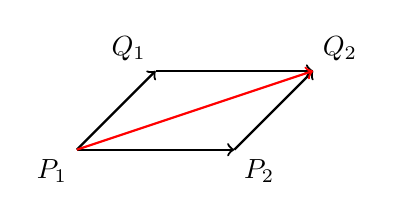
\begin{tikzpicture}
                \coordinate (P_1) at (0, 0);
                \coordinate (P_2) at (2, 0);
                \coordinate (Q_1) at (1, 1);
                \coordinate (Q_2) at (3, 1);
                \draw[thick, ->] (P_1) -- (P_2);
                \draw[thick, ->] (P_1) -- (Q_1);
                \draw[thick, ->] (Q_1) -- (Q_2);
                \draw[thick, ->] (P_2) -- (Q_2);
                \draw[red, thick, ->] (P_1) -- (Q_2);
                \node[below left] at (P_1) {\(P_1\)};
                \node[below right] at (P_2) {\(P_2\)};
                \node[above right] at (Q_2) {\(Q_2\)};
                \node[above left] at (Q_1) {\(Q_1\)};
            \end{tikzpicture}
        \end{center} 
\end{enumerate}
}

\dfn{Sottospazio affine}{Sia \(A_n(K)\) uno spazio affine. Si dice \textbf{sottospazio affine} di dimensione \(m \le n\) una struttura data da
\begin{enumerate}
    \item \(\emptyset \neq A' \subseteq A\), detto \textbf{sostegno del sottospazio affine} 
    \item \(V_m(K)\) sottospazio di \(V_n(K)\) 
    \item la restrizione dell'applicazione \(f\) ad \(A' \times A'\) troncata a \(V_m(K)\), purché questa sia ancora un'applicazione che gode delle proprietà elencate nella definizione di spazio affine
\end{enumerate}}

\dfn{Traslazione}{Fissato un vettore \(v \in V_n(K)\) si dice \textbf{traslazione}, individuata da \(v\), la corrispondenza \[
t_v: A \to A \quad e \quad P \to Q
\] che associa a un punto \(P \in A\) il punto \(Q\) traslato di \(P\) mediante il vettore \(v\).}

\paragraph{Osservazione:} \(\forall v \in V_n(K)\) la mappa \(t_v\) è una biiezione di \(A\), insieme di punti di \((A, V_n(K), f)\). E l'inversa di \(t_v\) è \(t_{-v}\).

\dfn{Sottospazio lineare}{Sia \(A_n(K)\) uno spazio affine. Si dice \textbf{sottospazio lineare} l'insieme dei traslati di un punto \(P\), detto \textbf{origine}, mediante i vettori \(v \in V_h(K) \le V_n(K)\), con \(h\) detta dimensione del sottospazio lineare. Inoltre si denota con \(S_h = [P, V_h(K)]\) il sottospazio lineare dato dal punto \(P\) e dallo spazio di traslazione \(V_h\).}

\dfn{Punti, rette, piani e iperpiani}{Sia \(A_n(K)\) uno spazio affine. Si dicono
\begin{itemize}
    \item \textbf{punti} i sottospazi lineari di dimensione 0 \[
            S_0 = [P, \{\ul{0} \} ] = \{P\} 
    \]
    \item \textbf{rette} i sottospazi lineari di dimensione 1 \[
            S_1 = [P, \mcL(v) ] \quad \text{con} \ v \neq \ul{0} \quad e \quad v \in V_n(K)
    \] 
    \item \textbf{piani} i sottospazi lineari di dimensione 2 \[
            S_2 = [P, \mcL(v_1, v_2) ] \quad \text{con} \ v_1, v_2 \neq \ul{0} \quad e \quad v_1, v_2 \in V_n(K)
    \] 
    \item \textbf{iperpiani} sono i sottospazi di dimensione \(n-1\)
\end{itemize}}
\mprop{}{Sia \(S_h = [P,V_h(K)]\) un sottospazio lineare di dimensione \(h\) sottospazio di \(A_n(K)\).
\begin{enumerate}
    \item siano \(Q, R \in S_h \implies \vec{QR} \in V_h(K)\) 
    \item se \(Q \in S_h\) e \(v \in V_h\), allora \(R = t_v (Q) \in S_h\)
\end{enumerate}}

\pf{Dimostrazione}{Dimostriamo entrambi i punti separatamente
\begin{enumerate}
    \item Per ipotesi \(Q \in S_h\), quindi \(Q = t_v(P)\) con \(v \in V_h(K)\). \(v = \vec{PQ} \in V_h\) e analogamente \(\vec{PR} \in V_h\). Ma allora \(\vec{QR} = \vec{QP} + \vec{PR} = - \vec{PQ} + \vec{PR} \in V_h\).
\begin{center}
        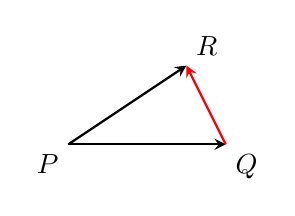
\begin{tikzpicture}
            \coordinate (P) at (0, 0);
            \coordinate (Q) at (2, 0);
            \coordinate (R) at (1.5, 1);
            \draw[thick, -stealth] (P) -- (R);
            \draw[thick, -stealth] (P) -- (Q);
            \draw[red, thick, -stealth] (Q) -- (R);
            \node[above right] at (R) {\(R\)};
            \node[below right] at (Q) {\(Q\)};
            \node[below left] at (P) {\(P\)};
        \end{tikzpicture}
\end{center}
    \item Poiché \(Q \in S_h, \ \vec{PQ} \in V_h\). Allora \(\vec{PR} + \vec{QR} = \vec{PQ} + \vec{v} \in V_h \implies \vec{PR} \in V_h\). Posto \(w = \vec{PR}\), \(t_w(P) = R\) con \(w \in V_h \implies R \in S_h\).
\begin{center}
        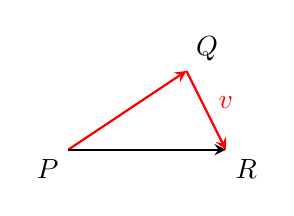
\begin{tikzpicture}
            \coordinate (P) at (0, 0);
            \coordinate (Q) at (2, 0);
            \coordinate (R) at (1.5, 1);
            \draw[red, thick, -stealth] (P) -- (R);
            \draw[thick, -stealth] (P) -- (Q);
            \draw[red, thick, -stealth] (R) -- (Q);
            \node[above right] at (R) {\(Q\)};
            \node[below right] at (Q) {\(R\)};
            \node[below left] at (P) {\(P\)};
            \node[red] at (2, 0.6) {\(v\)};
        \end{tikzpicture}
\end{center}
\end{enumerate}}

\mprop{}{Sia \(S_h=[P, V_h(K)]\) un sottospazio lineare di \(A_n(K)\). Ogni punto di \(S_h\) può essere scelto come origine di \(S_h\). Cioè dato \(Q \in S_h\) abbiamo che \([Q, V_h(K)] = S_h\).}

\pf{Dimostrazione}{Sia \(R \in S_h\). Allora \(\vec{PR} \in V_n\) e \(\vec{PQ}\in V_n\). Quindi \(\vec{QR} = \vec{QP} + \vec{PR} = - \vec{PQ} + \vec{PR} \in V_h \implies \vec{QR} \in V_h\).
\begin{center}
        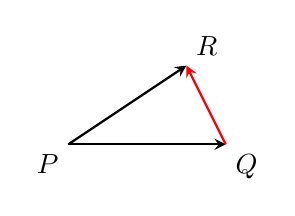
\begin{tikzpicture}
            \coordinate (P) at (0, 0);
            \coordinate (Q) at (2, 0);
            \coordinate (R) at (1.5, 1);
            \draw[thick, -stealth] (P) -- (R);
            \draw[thick, -stealth] (P) -- (Q);
            \draw[red, thick, -stealth] (Q) -- (R);
            \node[above right] at (R) {\(R\)};
            \node[below right] at (Q) {\(Q\)};
            \node[below left] at (P) {\(P\)};
        \end{tikzpicture}
\end{center}
Detto \(w = \vec{QR}\) abbiamo che \(R = t_v(Q)\). \(R\) è traslato di \(Q\) tramite il vettore \(w \in V_h \implies R \in [Q, V_h]\), quindi \[
    S_h \subseteq [Q, V_h]
\] con lo stesso ragionamento scambiamo \(P\) e \(Q\) si dimostra che  \[
[Q, V_h] \subseteq [P, V_h] = S_h
\] e ciò vale solo se \(S_h = [Q, V_h]\).}

\mprop{}{Siano \(S_h\) e \(S_k\) due sottospazi lineari di \(A_n(K)\). Allora \(S_h \subseteq S_k \iff S_h \cap S_k \neq \emptyset\) e \(V_h \le V_k\).}
\pf{Dimostrazione}{"\(\implies \)" Ovviamente \(S_h \cap S_k \neq \emptyset\) e sia \(P \in S_h \cap S_k\). Potremo scrivere \(S_h = [P, V_h]\) e \(S_k = [P, V_k]\). Sia \(v \in V_h\) e sia \(Q = t_v(P) \in S_h \subseteq S_k \implies Q \in S_k\) e sia \(Q = t_v(P)\) ovvero \(\vec{PQ}=v \in V_k \implies V_h \le V_k\).

"\(\impliedby \)" Sia \(P \in S_h \implies [P, V_h] \subseteq [P, V_k]\) (poiché per ipotesi \(V_h \subseteq V_k\)) \([P, V_h] = S_h\) e \([P, V_k]= S_k \implies S_h \subseteq S_k\).}

\mprop{}{Siano \(S_h\) e \(S_k\) sottospazi lineari di \(A_n(K)\). Sia \(S_h \cap S_k \neq \emptyset\) e sia \(P \in S_h \cap S_k\). Allora \[
        S_h \cap S_k = [P, V_h \cap V_k]
\] }

\pf{Dimostrazione}{Sia \(Q \in S_h \cap S_k\). Osserviamo che \(S_h = [P, V_h]\) e \(S_k = [P, V_k]\). \(Q = t_v(P)\) con \(v \in V_h\) (perché \(Q \in S_h\)). Ma \(Q = t_v(P)\) con \(v \in V_k\) (perché \(Q \in S_k\)). Quindi \(Q \in [P, V_h \cap V_k]\) perché \(v \in V_h \cap V_k\), cioè \[
        S_h \cap S_k \subseteq [P, V_h \cap V_k]
\] Viceversa dato \(Q = t_v(P)\) con \(v \in V_h \cap V_k \implies Q \) appartiene sia a \(S_h\) che ad \(S_k\), quindi \(Q \in S_h \cap S_k\), ovvero  \[
[P, V_h \cap V_k] \subseteq S_h \cap S_k
\] \[
\implies [P, V_h \cap V_k] = S_h \cap S_k
\] }

\dfn{Parallelismo tra sottospazi}{Due sottospazi lineari, \(S_p = [P, V_p]\) ed \(S_q = [Q, V_q]\), di \(A_n(K)\) si dicono \textbf{paralleli}, e si scrive \(S_p || S_q\), se i rispettivi spazi di traslazione sono confrontabili, ovvero quando \(V_p \subseteq V_q\), oppure \(V_q \subseteq V_p\).}

\paragraph{Osservazione 1:} La relazione di parallelismo non è transitiva. E' invece riflessiva e simmetrica. Non è quindi una relazione d'equivalenza.
\paragraph{Osservazione 2:} Due sottospazi lineari della stessa dimensione sono paralleli se, e soltanto se, hanno lo stesso spazio di traslazione. Quindi la relazione di parallelismo considerata tra spazi della stessa dimensione è una relazione d'equivalenza.

\mprop{}{Due sottospazi lineari paralleli e di uguale dimensione o coincidono oppure hanno intersezione vuota.}
\dfn{}{
\begin{itemize}
    \item Sia \(S=[P, V_1]\) una retta. Lo spazio \(V_1\) si dice \textbf{direzione} della retta \(S\). Quindi due rette sono parallele se, e soltanto se, hanno la stessa direzione
    \item Sia \(\pi = [P, V_2]\subseteq A_n(K)\) con \(n \ge 2\). Lo spazio \(V_2\) è detto \textbf{giacitura} di \(\pi\). Quindi due piani sono paralleli se, e soltanto se, hanno la stessa giacitura.
    \item Tre o più punti si dicono \textbf{allineati} se esiste una retta che li contiene tutti.
    \item Due o più rette si dicono \textbf{complanari} se esiste un piano che le contiene tutte.
\end{itemize}
}

\section{Proprietà di punti, rette e piani}
\mprop{}{In \(A_n(k)\), con \(n \ge 2\) 
\begin{enumerate}
    \item per ogni due punti distinti passa un'unica retta
    \item per due rette distinte, parallele o incidenti, passa un unico piano
    \item due rette complanari, aventi intersezione vuota, sono parallele
    \item per un punto passa un'unica retta parallela a una retta data (V Postulato di Euclide)
    \item per un punto passa un unico piano, parallelo ad un piano dato
    \item per tre punti, non allineati, passa un unico piano
    \item una retta, avente due punti distinti in un piano, giace nel piano
    \item per un punto passano almeno due rette distinte
\end{enumerate}}

\mprop{}{In \(A_3(K)\),
\begin{enumerate}
    \item una retta e un piano, aventi intersezione vuota, sono paralleli
    \item due piani, aventi intersezione vuota, sono paralleli
    \item due piani distinti, aventi in comune un punto, hanno in comune una retta per quel punto
    \item per una retta passano almeno due piani distinti
\end{enumerate}}

\dfn{Rette sghembe}{In \(A_n(K)\), con \(n \ge 3\), due rette non complanari si dicono \textbf{sghembe}.}
\mprop{}{In \(A_n(K)\), con \(n \ge 3\), esistono due rette \(r_1\) e \(r_2\) sghembe tra loro. Inoltre due rette sghembe \(r_1\) e \(r_2\), sono contenute su due piani \(\pi_1\) e \(\pi_2\) paralleli tra loro e distinti.}

\pf{Dimostrazione}{ Per ipotesi, \(A_n(K)\) ha dimensione almeno 3, quindi esistono nello spazio vettoriale  \(V_n(K)\) almeno 3 vettori linearmente indipendenti. Siano  essi \(u, v, w\). Siano inoltre, \(P\) un punto di \(A\) e \(Q\) il traslato di \(P\) mediante il vettore \(u\) (\(Q = t_u(P)\)). Dimostriamo che le rette \(r = [P, \mcL(v) ]\) ed \(s = [Q, \mcL(w) ]\) sono sghembe. Se infatti, esistesse un piano \(\pi = [P, V_2]\) che le contiene entrambe, lo spazio di traslazione di \(\pi \) conterrebbe 3 vettori linearmente indipendenti, cioè \(v, w\) e \(u = \vec{PQ}\) e ciò è un \textbf{assurdo!}
\begin{figure}[ht]
    \centering
    \def\svgwidth{0.3\columnwidth}
    \incfig{due-rette-complanari-con-3-vettori-linearmente-indipendenti}
    \label{fig:due-rette-complanari-con-3-vettori-linearmente-indipendenti}
\end{figure}
Siano ora \(t = [T, \mcL(v) ]\) e \(t' = [T', \mcL(v') ]\) due rette sghembe. I vettori \(v\) e \(v'\) generano uno spazio vettoriale \(V_2\) di dimensione 2. Pertanto, i piani  \(\pi = [T, V_2]\) e \(\pi' = [T', V_2]\), che risultano paralleli, sono distinti e contengono, rispettivamente le rette \(t\) e \(t'\).}

\section{Geometria analitica in \(A_n(\RR )\)}
\dfn{Riferimento affine}{Si dice \textbf{riferimento affine} di \(A_n(\RR )\) una coppia \(RA = [O,B]\) costituita da un punto \(O\) fissato, detto origine, e da una base \(B\) dello spazio vettoriale \(V_n(\RR )\).}

\dfn{Coordinate}{Fissato, in \(A_n(\RR )\), un riferimento affine \(RA = [O,B]\), si dicono \textbf{coordinate} del punto \(P\) in \(RA\) le componenti, in \(B\), del vettore \(\vec{OP}\) e si scrive \(P=(x_i)_{i \in I_n}\).}

\begin{enumerate}
\item In \(A_1(\RR )\), un riferimento affine è una coppia \(RA = [O,B]\), ove \(O\) è un punto fissato e \(B = (e_1)\) è una base di \(V_1(\RR )\). Se \(\vec{OP}=xe_1\), si scrive \(P=(x)\) e si dice che \(x\) è l'\textbf{ascissa} del punto \(P\) in \(RA\). 
\begin{figure}[ht]
    \centering
    \def\svgwidth{0.5\columnwidth}
    \incfig{ascissa}
    \label{fig:ascissa}
\end{figure}
\item In \(A_2(\RR )\), un riferimento affine è una coppia \(RA = [O,B]\), ove \(O\) è un punto fissato e \(B = (e_1, e_2)\) è una base di \(V_2(\RR )\). La retta \([O, \mcL(e_1) ]\) è detta \textbf{asse delle ascisse} e la retta \([O, \mcL(e_2) ]\) è detta \textbf{asse delle ordinate}. Se \(\vec{OP} = xe_1 + y e_2\), si scrive \(P = (x, y)\) e si dice che \((x,y)\) è la coppia delle coordinate di \(P\) in \(RA\), dette rispettivamente \textbf{ascissa} e \textbf{ordinata} del punto \(P\).
\begin{figure}[ht]
    \centering
    \def\svgwidth{100pt}
    \incfig{ascissa-e-ordinata}
    \label{fig:ascissa-e-ordinata}
\end{figure}
\item In \(A_3(\RR )\), un riferimento affine è una coppia \(RA = [O,B]\), ove \(O\) è un punto fissato e \(B = (e_1, e_2, e_3)\) è una base di \(V_3(\RR )\). La retta \([O, \mcL(e_1) ]\) è detta \textbf{asse delle ascisse}, la retta \([O, \mcL(e_2) ]\) è detta \textbf{asse delle ordinate} e la retta \([O, \mcL(e_3) ]\) è detta \textbf{asse delle quote}. Sono detti \textbf{piani coordinati} i piani \(xy = [O, \mcL(e_1, e_2) ], xz = [O, \mcL(e_1, e_3) ]\) e \(yz = [O, \mcL(e_2, e_3) ]\). Inoltre, se \(\vec{OP}=xe_1+ ye_2 + ze_3\), si scrive \(P = (x, y,z)\) e si dice che \((x, y, z)\) è la terna delle coordinate di \(P\) in \(RA\), dette rispettivamente \textbf{ascissa, ordinata} e \textbf{quota} del punto \(P\).
\begin{figure}[ht]
    \centering
    \def\svgwidth{200pt}
    \incfig{terne-di-coordinate}
    \label{fig:terne-di-coordinate}
\end{figure}
\end{enumerate}

\thm{}{In \(A_n(K)\), con \(RA = [O, B]\), siano \(P = (x_1', x_2', \ldots , x_n')\) e \(Q = (x_1 '', x_2 '', \ldots  , x_n '')\) due punti di \(A\). Allora le componenti di \(\vec{PQ}\) rispetto a \(B\) sono \[
(x_1 '' - x_1', x_2 '' - x_2' , \ldots, x_n '' - x_n')
\] }

\pf{Dimostrazione}{Posti due vettori \[
\vec{OP} : \ x_1' e_1+ x_2' e_2 + \ldots + x_n' e_n
\] \[
\vec{OQ}: \ x_1 '' e_1 + x_2 '' e_2 + \ldots + x_n '' e_n
\]Per la proprietà della definizione di spazio affine possiamo dire che \[
\vec{PQ} = \vec{PO} + \vec{OQ} = \vec{OQ} - \vec{OP} = \sum_{i \in I_n} (x_i '' - x_i') e_i
\] }
Posti \[
 X '' = \left( \; \begin{matrix} x ''_1 \\ x ''_2\\ \vdots \\ x ''_n \end{matrix} \; \right), X' = \left( \; \begin{matrix} x'_1 \\ x'_2\\ \vdots \\ x'_n \end{matrix} \; \right) \text{ e } T = \left( \; \begin{matrix} t_1 \\ t_2\\ \vdots \\ t_n \end{matrix} \; \right)
\] si ottiene l'equivalente, ma spesso più agevole, forma matriciale: \[
X '' - X' = T
\] che può essere riscritta come \[
X '' = X' + T
\] Da quest'ultima equazione si vede che le coordinate del traslato del punto \(P = (x_1', x_2', \ldots , x_n')\), attraverso il vettore \(v\) di componenti \((t_1, t_2, \ldots , t_n)\), si ottengono sommando, ordinatamente, alle coordinate di \(P\) le componenti del vettore di traslazione. Per questo le relazioni che compaiono nell'equazione sono anche dette \textbf{equazioni della traslazione individuata da \(v\)}.

\dfn{Punto medio}{Dato \(P\) e \(Q \in A\) (insieme dei punti di \(A_n(\RR )\)), definiamo il punto medio del segmento \([PQ]\) come \[
M = t_{1/2 \vec{PQ}} (P)
\] 
\begin{center}
    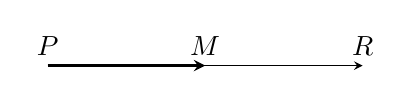
\begin{tikzpicture}
        \coordinate (P) at (0, 0);
        \coordinate (M) at (2, 0);
        \coordinate (R) at (4, 0);
        \draw[thick, -stealth] (P) -- (M);
        \draw[thin, -stealth] (P) -- (R);
        \node[above] at (R) {\(R\)};
        \node[above] at (M) {\(M\)};
        \node[above] at (P) {\(P\)};
    \end{tikzpicture}
\end{center}}

\mprop{}{Dati \(P, Q \in A\) e dato un riferimento affine \(RA = [O, B]\) abbiamo che le coordinate del punto medio di \(P\) e \(Q\) sono le semisomme delle coordinate omonime di \(P\) e di \(Q\).}

\dfn{Punto simmetrico}{In \(A_n(\RR )\) dati i punti \(P\) e \(C\) diremo che \(S\) è il \textbf{punto simmetrico} di \(P\) rispetto a \(C\) se \(C\) è il punto medio di \([P, S]\).}

\section{Rappresentazioni analitiche}
\dfn{Equazioni parametriche di una retta in \(A_n(\RR )\)}{Sia \(RA = [O,B]\) un riferimento fissato in \(A_n(\RR )\), ove \(B = (e_1, e_2, \ldots , e_n)\). Sia \(r = [P, V_1 = \mcL(v) ]\) la retta di origine il punto \(P = (x_1', x_2', \ldots , x_n')\) e spazio di traslazione generato da \(v = (l_1, l_2, \ldots , l_n)\). Il generico vettore \(w\) di \(\mcL(v) \) è proporzionale al vettore \(v\), cioè \(w = tv\), con \(t \in \RR \), quindi, \(w = (tl_1, tl_2, \ldots , tl_n)\). Dato che la retta \(r\) è il luogo dei traslati di \(P\) attraverso i vettori di \(\mcL(v) \), applicando le equazioni del teorema precedente si ottengono le coordinate del generico punto di \(r\) \[
\begin{cases}
    \ x_1 = x_1' + l_1t \\
    \ x_2 = x_2' + l_2t \\
    \ \ldots \ldots \ldots \ldots \\
    \ x_n = x_n' + l_nt \\
\end{cases} \quad \text{con} \quad t \in \RR , \quad (l_1, l_2, \ldots , l_n) \neq \ul{0} 
\] tali equazioni sono dette \textbf{equazioni parametriche} di \(r\) in \(A_n(\RR )\). Al variare di \(t \in \RR \), si ottengono le coordinate di tutti i punti di una retta e, quindi, tutti i punti di una retta sono \(\infty^{1}\).}

\dfn{Parametri direttori}{Si dicono \textbf{parametri direttori} di \(r = [P, V_1]\), le componenti di un qualunque vettore nullo di \(V_1\).}
\paragraph{Osservazione:} I parametri direttori di una retta sono, quindi, determinati a meno di un fattore non nullo di proporzionalità. Definiamo la classe dei parametri direttori di \(r\) come \(p.d.r = [(l_1, l_2, \ldots , l_n)]\) con \((l_1, l_2, \ldots , l_n)\) un qualsiasi vettore appartenente a \(V_1\).

\subsubsection{Equazioni parametriche di una retta in \(A_2(\RR )\)} 
In \(A_2(\RR )\), sia fissato un riferimento \(RA = [O, B]\), ove \(B = (e_1, e_2)\). Una retta \(r = [P, V_1]\) è il luogo dei traslati di un punto \(P\) mediante i vettori di \(V_1 \subset V_2\). Se \(P\) ha coordinate \((x_0, y_0)\) e \(V_1 = \mcL(v) \), ove \(v = le_1 + me_2\), le equazioni della definizione diventano \[
\begin{cases}
    \ x = x_0 + lt \\
    \ y = y_0 + mt \\
\end{cases}
\quad \text{ove}\quad t \in \RR , \quad (l,m) \neq (0,0)\] 
e sono dette \textbf{equazioni parametriche} di \(r\) in \(A_2(\RR )\).

\subsubsection{Equazioni parametriche di una retta in \(A_3(\RR )\)}
In \(A_3(\RR )\), sia fissato un riferimento \(RA = [O, B]\), ove \(B = (e_1, e_2, e_3)\). Una retta \(r = [P, V_1]\) è il luogo dei traslati di un punto \(P\) mediante i vettori di \(V_1 \subset V_3\). Se \(P\) ha coordinate \((x_0, y_0, z_0)\) e \(V_1 = \mcL(v) \), ove \(v = le_1 + me_2 + ne_3\), le equazioni della definizione diventano \[
\begin{cases}
    \ x = x_0 + lt \\
    \ y = y_0 + mt \\
    \ z = z_0 + nt \\
\end{cases}
\quad \text{ove}\quad t \in \RR , \quad (l,m,n) \neq (0,0,0)\] 
e sono dette \textbf{equazioni parametriche} di \(r\) in \(A_3(\RR )\).

\paragraph{Osservazione:} In modo del tutto analogo possiamo determinare le equazioni parametriche di sottospazi lineari di dimensione \(n\), che quindi dipenderanno da \(n\) parametri.

\subsubsection{Equazione cartesiana di una retta in \(A_2(\RR )\)}
In \(A_2(\RR )\) una retta si può rappresentare attraverso le sue equazioni parametriche in questo modo \[
\begin{cases}
    \ x = x_p + lt \\
    \ y = y_p + mt \\
\end{cases}
\] possiamo convertire questo sistema lineare in forma matriciale e quindi \[
\left( \;
\begin{matrix}
    x \\
    y \\
\end{matrix} \;
\right) = 
\left( \; \begin{matrix}
    x_p \\
    y_p \\
\end{matrix} \; \right) +
t  
\left( \; \begin{matrix}
    l \\
    m \\
\end{matrix} \; \right) \iff 
\left( \; \begin{matrix}
    x - x_p \\
    y - y_p \\
\end{matrix} \; \right) = t
\left( \; \begin{matrix}
    l \\
    m \\
\end{matrix} \; \right) \iff 
\left| \;
\begin{matrix}
    x - x_p & y - y_p \\
    l & m \\
\end{matrix} \;
\right| = 0
\] 
Quindi vale la relazione \[
    ((x-x_p) m) (l (y-y_p)) = mx - ly -mx_p + ly_p = 0
\] Possiamo raggruppare i termini noti \(-mx_p + ly_p\) in un generico termine \(c\) e quindi l'equazione cartesiana della retta diventa \[
ax + by + c = 0 \quad \text{con}\quad (a,b) \neq (0,0)
\] Quindi i parametri direttori della generica retta \(r\) saranno \(p.d.r = [(l,m)] = [(-b, a)]\).

\subsubsection{Mutua posizione di due rette in \(A_2(\RR )\)}
Siano due rette \[
r: ax + by + c = 0 \quad (a,b) \neq (0,0)
\] \[
s: a'x + b'y + c' = 0 \quad (a', b') \neq (0,0)
\]
La loro intersezione può essere \[ r \cap s = \
\begin{cases}
    \ \text{un unico punto se \(r\) e \(s\) sono incidenti} \\
    \ \emptyset \text{ se \(r\) e \(s\) sono parallele e distinte} \\
    \ r \equiv s \text{ se sono coincidenti } \\
\end{cases}
\]
Consideriamo il sistema \[r \cap s=
\begin{cases}
    \ ax + by + c = 0 \\
    \ a'x + b'y + c' = 0 \\
\end{cases}
\]
Le coordinate dei punti di \(r \cap s\) sono le soluzioni del sistema. Posti \[
A =
\left( \; \\
 \begin{matrix}
    a & b \\
    a' & b' \\
\end{matrix} \; \\
 \right) \quad \text{la matrice incompleta del sistema,}
 \quad A|B =
\left( \; \\
 \begin{matrix}
    a & b & -c \\
    a' & b' & -c' \\
\end{matrix} \; \\
 \right) \quad \text{la matrice completa del sistema}
\] possiamo dire che \(\rho(A) \ge 1\) poiché abbiamo richiesto che \((a,b) \neq (0,0)\) e \(\rho(A) \le 2\). Quindi abbiamo due casi possibili
\begin{enumerate}
    \item se \(\rho(A) = 2 \implies \rho(A) = \rho(A|B) =2\), quindi il sistema è compatibile e ha \(\infty^{2-2}\) soluzioni \(\implies \exists !\) soluzione del sistema \(\implies r \cap s = \{P\} \implies r \cap s\) sono \textbf{incidenti}.
    \item se \(\rho(A) = 1\) allora \(r || s\), ma non sappiamo se esse siano parallele e distinte o se esse coincidano. Perciò dobbiamo suddividere in due sottocasi
        \begin{enumerate}
            \item se fossero parallele e distinte il sistema non sarebbe compatibile, perciò \(2= \rho(A|B) > \rho(A) = 1\)
            \item se invece \(\rho(A) = 1\) e \(\rho(B) = 1\) il sistema ammette \(\infty^{2-1}\) soluzioni, perciò \(r \equiv s \implies r||s\) se \(\rho(A) = 1\)
        \end{enumerate}
\end{enumerate}
\subsubsection{Fasci di rette in \(A_2(\RR )\)}
\dfn{Fascio improprio di rette}{Si dice \textbf{fascio improprio di rette} l'insieme di tutte e sole le rette del piano \(A_2(\RR )\) parallele ad una retta data.}
\mprop{}{Una retta appartiene al fascio improprio di rette parallele alla retta \(r = [P, V_1]: ax + by + c = 0, \ (a,b) \neq (0,0)\), se, e soltanto se, ha un'equazione del tipo \[
ax + by + k = 0 \quad \text{ove} \quad k \in \RR 
\] detta \textbf{equazione del fascio improprio di rette}. Da cui si deduce che le rette di un fascio improprio di rette sono \(\infty^{1}\)}
\paragraph{Osservazione:} Tutte e sole le rette parallele ad \(r\) hanno parametri direttori \([(-b, a)]\) e quindi \(r\) e \(s\) sono la stessa retta \(\iff (a,b,c) \sim (a',b', c')\).

\dfn{Fascio proprio di rette}{Si dice \textbf{fascio proprio di rette} l'insieme di tutte le rette di \(A_2(\RR )\) passanti per un punto \(P\) dato, detto \textbf{centro} o \textbf{sostegno} del fascio.}

\mprop{}{Siano \(r: ax + by + c = 0\) e \(r': a'x + b'y + c' = 0\), con \((a,b) \neq (0,0)\) e \((a', b') \neq (0,0)\), due distinte rette incidenti in un punto \(P\). Una retta \(s\) appartiene al fascio di centro \(P\) se, e soltanto se, ha un'equazione di tipo \[
\lambda (ax + by + c) + \mu(a'x+ b'y + c') = 0 \quad \text{ove} \quad \lambda , \mu \in \RR \quad e \quad (\lambda , \mu) \neq (0,0)
\] detta \textbf{equazione del fascio proprio di rette}. Se nell'equazione risulta \(\lambda  \neq 0\), posto \(k = \mu / \lambda \), si ottiene \[
ax + by + c + k (a'x + b'y + c') = 0 \quad \text{ove} \quad k \in \RR 
\] detta \textbf{equazione ridotta del fascio proprio di rette}, in cui, ovviamente, la retta \(r' : a'x + b'y + c' = 0\) non è rappresentata. Quindi possiamo dire che le rette di un fascio proprio di rette sono \(\infty^{1}\).}

\subsubsection{Simmetrie in \(A_2(\RR )\)}
\dfn{Simmetria rispetto ad una retta}{Il punto \(T\) si dice \textbf{simmetrico} del punto \(H\), rispetto alla retta \(r = [P, V_1]\), detta \textbf{asse di simmetria}, nella direzione \(W_1 \neq V_1\), se lo è nella simmetria di centro \(C = r \cap s\), dove \(s = [H, W_1]\). Tale simmetria si dice anche \textbf{simmetria rispetto ad una retta in una direzione assegnata}.}

\begin{figure}[ht]
    \centering
    \def\svgwidth{160pt}
    \incfig{simmetria-punto-retta}
    \label{fig:simmetria-punto-retta}
\end{figure}

\subsubsection{Equazione cartesiana di un piano in \(A_3(\RR )\)}
In \(A_3(\RR )\) dato il \(RA = [O, B]\), con \(B = (e_1, e_2, e_3)\). Sia \(\alpha = [P, V_2]\) un piano con \(P = (x_p, y_p, z_p)\) e \(V_2 = \mcL(v, v') \) (con \(v \neq kv'\)), tali che  \[
v = le_1 + me_2 + ne_3 \qquad 
v' = l'e_1 + m'e_2 + n'e_3
\] 
Il generico vettore \(w \in V_2\) si scrive come \(w = tv + t' v'\). Quindi \(t_w(P)\) è il generico punto appartenente a \(\alpha \). Di conseguenza possiamo dire che \[
\begin{cases}
    \ x = x_p + tl + t'l' \\
    \ y = y_p + tm + t'm' \\
    \ z = z_p + tn + t'n' \\
\end{cases} \implies 
\left( \;
 \begin{matrix}
    x \\
    y \\
    z \\
\end{matrix} \;
 \right) =
\left( \;
 \begin{matrix}
    x_p \\
    y_p \\
    z_p \\
\end{matrix} \;
 \right) +
\left( \;
 \begin{matrix}
    tl + t'l' \\
    tm + t'm' \\
    tn + t'm' \\
\end{matrix} \;
 \right) 
\] cioè, per l'equazione della traslazione \(\left( \; \begin{matrix} x \\ y\\ z \end{matrix} \; \right) \) sono le coordinate del generico punto di \(\alpha \). Date dalla somma di \(\left( \; \begin{matrix} x_p \\ y_p\\ z_p \end{matrix} \; \right) \) cioè le coordinate di \(P\) con \(\left( \; \begin{matrix} tl + t'l' \\ tm + t'm'\\ tn + t'n' \end{matrix} \; \right) \) cioè le componenti di \(w\).

Seguendo un ragionamento analogo a quello fatto per le rette in \(A_2(\RR )\) possiamo descrivere un piano in \(A_3(\RR )\) come \[
\left| \; \begin{matrix}
    x-x_p & y-y_p & z-z_p \\
    l & m & n \\
    l' & m' & n' \\
\end{matrix} \; \right| = 0
\] e da questa ne ricaviamo la seguente equazione \[
ax + by + cz + d = 0 \quad \text{con} \quad  (a,b,c) \neq (0,0,0)
\] detta \textbf{equazione cartesiana} del piano in \(A_3(\RR )\). Tale equazione è definita a meno di un fattore di proporzionalità non nullo.

\subsubsection{Equazioni cartesiane delle rette in \(A_3(\RR )\)}

Fissiamo un \(RA = [O, B]\) con \(B = (e_1, e_2, e_3)\) e data una retta \(r = [P, V_1=\mcL(l,m,n) ]\) possiamo scrivere l'equazione parametrica della retta \[
r : \
\begin{cases}
    \ x = x_p + tl \\
    \ y = y_p + tm \\
    \ z = z_p + tn \\
\end{cases} \quad \text{con}\quad (l,m,n) \neq (0,0,0)
\] Da cui deriva la seguente relazione \[
\frac{x-x_p}{l} = \frac{y-y_p}{m} = \frac{z - z_p}{n}
\] in particolare, se poniamo ad esempio \(l \neq 0\), otteniamo il seguente sistema \[
\begin{cases}
    \ y = \frac{m}{l} (x-x_p) + y_p \\
    \ z = \frac{n}{l} (x-x_p) + z_p \\
\end{cases} \implies 
\begin{cases}
    \ y = \frac{m}{l} x + k \\
    \ z = \frac{n}{l} x + h \\
\end{cases} \ \text{ove} \quad h, k \in \RR 
\] esistono, ovviamente le equazioni relative ai casi \(m \neq 0\) e \(n \neq 0\) e, dato che la terna \((l,m,n)\) è non nulla, ogni retta ammette sempre, almeno, una rappresentazione simile. In ogni caso, qualunque essa sia, possiamo concludere che una retta si rappresenta con un sistema di due equazioni lineari nelle incognite \(x, y\) e \(z\), in cui il rango della matrice incompleta è uguale a 2. E infatti sussiste anche il viceversa, cioè \[
\begin{cases}
    \ ax + by + cz + d = 0 \\
    \ a'x + b'y + c'z + d' = 0 \\
\end{cases} \ \text{con} \quad \rho
\left( \; \begin{matrix}
    a & b & c \\
    a' & b' & c' \\
\end{matrix} \; \right) = 2
\] rappresenta una retta. Infatti per il teorema di Rouché-Capelli il sistema è compatibile e ammette \(\infty^{1}\) soluzioni, cioè le sue soluzioni dipendono da un solo parametro.  

Analogamente a quanto già osservato in \(A_2(\RR )\), dalla precedente equazione deriva che le componenti, dei vettori dello spazio di traslazione della retta \(r\), sono le soluzioni del sistema omogeneo associato a una rappresentazione cartesiana di \(r\) stessa. Quindi possiamo dedurre la classe dei parametri direttori della retta \(r\) attraverso la regola dei minori. L'insieme delle \(\infty^{1}\) soluzioni del sistema omogeneo \[
\begin{cases}
    \ ax + by + cz + d = 0 \\
    \ a'x + b'y + c'z + d' = 0 \\
\end{cases} \ \text{con} \quad \rho
\left( \; \begin{matrix}
    a & b & c \\
    a' & b' & c' \\
\end{matrix} \; \right) = 2
\] è \[
\left\{ \left( t
\left| \; \begin{matrix}
    b & c \\
    b' & c' \\
\end{matrix} \; \right|,
-t
\left| \; \begin{matrix}
    a & c \\
    a' & c' \\
\end{matrix} \; \right|, t
\left| \; \begin{matrix}
    a & b \\
    a' & b' \\
\end{matrix} \; \right| \right)
: \ t \in R \right\}
\] 
\subsubsection{Mutua posizione di due piani in \(A_3(\RR )\)}
Fissato un \(RA\) e dati due piani in \(A_3(\RR )\)\[
\alpha : ax + by + cz + d = 0 \qquad \alpha' : a'x + b'y + c'z + d' = 0
\] la loro intersezione è data dal sistema \[
\alpha \cap \alpha' : \
\begin{cases}
    \ ax + by + cz + d = 0 \\
    \ a'x + b'y + c'z + d' = 0 \\
\end{cases}
\] Quindi possiamo distinguere in 3 casi:
\begin{enumerate}
    \item \(\rho(A) = 2 \implies \rho(A) = \rho(A|B) = 2 \) quindi il sistema è compatibile e ammette \(\infty^{3-2} = \infty^{1}\) soluzioni \(\implies \alpha \cap \alpha' = r\), quindi \(\alpha \) e \(\alpha'\) sono due piani \textbf{incidenti}.
    \item Nel caso in cui \(\rho(A) = 1\) dobbiamo distinguere in due sottocasi
        \begin{enumerate}
            \item \(\rho(A|B) = 2 \) e \(\rho(A) = 1\), il sistema non è compatibile, quindi \(\alpha \cap \alpha' = \emptyset\) e \(\alpha \) è parallelo e distinto da \(\alpha'\). \(\alpha \) e \(\alpha'\) sono detti \textbf{paralleli e distinti}.
            \item \(\rho(A) = 1\) e \(\rho(A|B) = 1\), il sistema è compatibile e ammette \(\infty^{3-1} = \infty^{2}\) soluzioni. Quindi l'insieme delle soluzioni dipende da due parametri \(\implies \alpha \equiv \alpha'\).
        \end{enumerate}
\end{enumerate}

\mprop{Condizione di parallelismo tra piani}{\(\alpha || \alpha' \iff \rho(A) = 1 \iff a = ka' \ b = kb' \ c = kc' \iff [(a,b,c)] = [(ka',kb',kc')] = [(a', b', c')]\). Questa viene denominata condizione analitica di parallelismo tra piani.}

\subsubsection{Fasci di piani in \(A_3(\RR )\)}
\dfn{Fascio improprio di piani}{Si dice \textbf{fascio improprio di piani} l'insieme di tutti e soli i piani di \(A_3(\RR )\) paralleli a un piano dato.}
\mprop{}{Un piano appartiene al fascio improprio di piani paralleli ad \(\alpha =[P, V_2]: ax + by + cz + d = 0\), con \((a,b,c) \neq (0,0,0)\), se, e soltanto se, ha un'equazione del tipo \[
ax + by + cz + k = 0 \quad \text{ove} \quad k \in \RR 
\] detta \textbf{equazione del fascio improprio di piani}. I piani di un fascio improprio sono \(\infty^{1}\).}

\dfn{Fascio proprio di piani}{Si dice \textbf{fascio proprio di piani}, l'insieme di tutti e soli i piani di \(A_3(\RR )\) passanti per una retta data \(r\), detta \textbf{asse} o \textbf{sostegno} del fascio.}
\mprop{}{Siano \(r\) una retta, \(\alpha : ax + by + cz + d = 0\) e \(\alpha' : a'x + b'y + c'z + d' = 0\), con \((a,b,c) \neq (0,0,0)\) e \((a',b',c') \neq (0,0,0)\), due distinti piani per \(r\). Un piano \(\beta \) appartiene al fascio di sostegno \(r\) se, e soltanto se, ha un'equazione del tipo \[
\lambda (ax+by+cz+d) + \mu (a'x + b'y +c'z+d') = 0 \quad \text{ove}\quad \lambda , \mu \in \RR \quad e \quad (\lambda , \mu) \neq (0,0)
\] detta \textbf{equazione del fascio proprio di piani}. Se nell'equazione risulta \(\lambda \neq 0\), posto \(h = \mu / \lambda \), si ottiene \[
ax + by + cz + d + h(a'x + b'y + c'z + d') = 0 \quad \text{ove} \quad h \in \RR 
\] detta \textbf{equazione ridotta del fascio proprio di piani}, in cui ovviamente il piano \(\beta : a'x + b'y + c'z + d' = 0\) non è rappresentato. Dalla rappresentazione ridotta del fascio si deduce che i piani di un fascio proprio sono \(\infty^{1}\).}

\subsubsection{Mutua posizione di due rette in \(A_3(\RR )\)}
Siano assegnate le rette \[
r :
\begin{cases}
    \ ax + by + cz + d = 0 \\
    \ a'x + b'y + c'z + d' = 0 \\
\end{cases} \quad \rho
\left( \; \begin{matrix}
    a & b & c \\
    a' & b' & c' \\
\end{matrix} \; \right) = 2
\] \[
s :
\begin{cases}
    \ a ''x + b ''y + c ''z + d '' = 0 \\
    \ a'''x + b'''y + c'''z + d''' = 0 \\
\end{cases} \quad \rho
\left( \; \begin{matrix}
    a ''& b '' & c ''\\
    a''' & b''' & c''' \\
\end{matrix} \; \right) = 2
\] Sia \[
r \cap s:
\begin{cases}
    \ ax + by + cz + d = 0 \\
    \ a'x + b'y + c'z + d' = 0 \\
    \ a ''x + b ''y + c ''z + d '' = 0 \\
    \ a'''x + b'''y + c'''z + d''' = 0 \\
\end{cases}
\] il sistema costituito dalle loro equazioni e siano \(A\) e \(A|B\) le matrici incompleta e completa associate al sistema. \[
AX = B \quad \text{con} \quad B =
\left( \; \begin{matrix}
    -d \\
    -d' \\
    -d'' \\
    -d''' \\
\end{matrix} \; \right) 
\quad X = 
\left( \; \begin{matrix}
    x \\
    y \\
    z \\
\end{matrix} \; \right) 
\quad A =
\left( \; \begin{matrix}
    a & b & c \\
    a' & b' & c' \\
    a '' & b '' & c '' \\
    a''' & b''' & c''' \\
\end{matrix} \; \right) 
\] Esaminiamo i 4 casi possibili:

\begin{enumerate}
    \item \(\rho(A|B) = 4 \implies \rho(A) = 3\) poiché \(A|B\) è ottenuta aggiungendo una colonna ad \(A\), quindi \(\rho(A|B) \le \rho(A) + 1 \implies \rho(A) =3 \). Il sistema non è compatibile per il teorema di Rouché-Capelli \(\implies r  \) e \(s\) sono o parallele e disgiunte, oppure sghembe. Ma siccome \(\rho(A) = 3 \implies r = [P,V_1] \quad s =[P', V_1'] \quad V_1 \neq V_1' \implies r\) non è parallela ad \(s\). Quindi \(r\) e \(s\) sono \textbf{sghembe}.
    \item \(\rho(A|B) = 3\) e \(\rho(A) =3\). Il sistema è compatibile e per il teorema di Rouché-Capelli  esiste un'unica soluzione \(r \cap s = \{P\} \implies r\) e \(s\) si dicono \textbf{incidenti}.
    \item \(\rho(A|B) = 3\) e \(\rho(A) = 2\). Il sistema non è compatibile per il teorema di R.C. Siccome \(\rho(A) =2 \implies V_1= V_1' \implies r\) è parallela a \(s\) e \(r \neq s\). Si dice che \(r\) e \(s\) sono \textbf{parallele e distinte}.
    \item \(\rho(A|B) = \rho(A) = 2\) il sistema è compatibile e ammette \(\infty^{1}\) soluzioni. Si dice che  le rette \(r\) e \(s\) sono \textbf{coincidenti}.
\end{enumerate}

\dfn{Stella propria di rette}{In \(A_3(\RR )\) si dice \textbf{stella propria} di rette, l'insieme di tutte e sole le rette passanti per un ponto assegnato.}
\paragraph{Osservazione:} Possiamo scrivere la rappresentazione di tutte e sole le rette della stella passanti per \(P = (x_0, y_0, z_0)\) come \[
\alpha :
\begin{cases}
    \ x = x_0 + tl \\
    \ y = y_0 + tm \\
    \ z = z_0 + tn \\
\end{cases}
\] e da qui abbiamo che \[
t = \frac{x-x_0}{l}= \frac{y-y_0}{m} = \frac{z-z_0}{n} = 
\begin{cases}
    \ m(x-x_0) = l(y-y_0) \\
    \ n (x-x_0) = l(z-z_0) \\
\end{cases}
\] dividendo per \(l\) (supponendo \(l \neq 0\)) si ottiene che abbiamo solo due parametri liberi e quindi abbiamo \(\infty^{2}\) rette nella stella di rette per \(P\).

\dfn{Stella impropria di rette}{In \(A_3(\RR )\) si dice \textbf{stella impropria} di rette, l'insieme di tutte e sole le rette parallele ad una retta data.}

\paragraph{Osservazione:} Una rappresentazione analitica di tutte le rette parallele a una retta assegnata, di parametri direttori \((l,m,n)\), è \[
\beta : 
\begin{cases}
    \ x = x' + tl \\
    \ y = y' + tm \\
    \ z = z' + tn \\
\end{cases} \iff  
\begin{cases}
    \ m(x-x') = l(y-y') \\
    \ n(x-x') = l(z-z') \\
\end{cases}
\] Questa volta non sono i parametri direttori ad essere i parametri, ma i punti di \(P = (x', y', z')\). Quest'ultima è detta \textbf{equazione cartesiana della stella impropria} di \(r\). Abbiamo \(\infty^2\) rette in \(A_3(\RR )\) parallele ad una retta data.

\subsubsection{Mutua posizione di due piani in \(A_3(\RR )\)}
Siano \[
\alpha = [P, V_2]: ax + by + cz + d = 0, \quad \text{con}\quad (a,b,c) \neq (0,0,0) \]
\[
r=[Q, V_1]:
\begin{cases}
    \ a'x + b'y + c'z + d' = 0 \\
    \ a ''x + b ''y + c ''z + d '' = 0 \\
\end{cases} \text{con} \quad 
\rho
\left( \; \begin{matrix}
    a' & b' & c' \\
    a '' & b '' & c '' \\
\end{matrix} \; \right) = 2
\] e sia \(r \cap \alpha \) rappresentato dal sistema lineare \(AX = B\), dove \[
A =
\left( \; \begin{matrix}
    a & b & c \\
    a' & b' & c' \\
    a '' & b '' & c '' \\
\end{matrix} \; \right) \quad
B =
\left( \; \begin{matrix}
    -d \\
    -d' \\
    -d '' \\
\end{matrix} \; \right) \quad X =
\left( \; \begin{matrix}
    x \\
    y \\
    z \\
\end{matrix} \; \right) 
\] Sono 3 i casi possibili
\begin{enumerate}
    \item sia \(\rho(A|B) = \rho(A) =3\), il sistema è compatibile e, per il teorema di R.C. ammette un'unica soluzione \(r \cap \alpha  = \{P\} \implies r\) e \(\alpha \) si dicono \textbf{incidenti}
    \item \(\rho(A|B) = 3\) e \(\rho(A) =2\), il sistema non è compatibile, quindi \(r || \alpha \) e \(r \notin \alpha \) 
    \item \(\rho(A|B) = 2\) e \(\rho(A) = 2\), il sistema è compatibile e ammette \(\infty^{1}\) soluzioni, quindi \(r\) è contenuto in \(\alpha \)(\(r\) è anche chiaramente parallelo ad \(\alpha \))
\end{enumerate}

\paragraph{Osservazione:} \(\rho(A) = 2 \iff r || \alpha \) ovvero \[
\left| \; \begin{matrix}
    a & b & c \\
    a' & b' & c' \\
    a '' & b '' & c '' \\
\end{matrix} \; \right| = 0 \iff 
a \underbrace{
\left| \; \begin{matrix}
    b' & c' \\
    b '' & c '' \\
\end{matrix} \; \right|
}_{ \Gamma_1 \to l } 
- b 
\underbrace{
\left| \; \begin{matrix}
    a' & b' \\
    a '' & c '' \\
\end{matrix} \; \right| 
}_{\Gamma_2 \to m} 
+ c
\underbrace{
\left| \; \begin{matrix}
    a' & b' \\
    a '' & b '' \\
\end{matrix} \; \right|
}_{\Gamma_3 \to n} = 0
\] Quindi posti i parametri direttori \([(l,m,n)]\) possiamo dare la
\mprop{Condizione di parallelismo tra retta e piano}{La condizione di parallelismo tra retta e piano si esprime come \[
al + bm + cn = 0
\] dove \([(l,m,n)]\) sono i parametri direttori della retta e il piano è \(ax + by + cz + d = 0\).}

\dfn{Stella impropria di piani}{Si dice \textbf{stella impropria di piani} l'insieme di tutti e soli i piani di \(A_3(\RR )\) paralleli ad una retta data.}
\paragraph{Osservazione:} Chiaramente dalla proposizione precedente segue che dati parametri direttori \([(l,m,n)]\) abbiamo che esistono \(\infty^{2}\) piani appartenenti alla stella impropria di piani.

\dfn{Stella propria di piani}{Si dice \textbf{stella propria di piani} l'insieme di tutti e soli i piani di \(A_3(\RR )\) passanti per un punto  assegnato detto \textbf{centro} o \textbf{sostegno} della stella.}
\paragraph{Osservazione:} Analogamente abbiamo \(\infty^{2}\) piani nella stella propria di piani.

\subsubsection{Simmetrie in \(A_3(\RR )\)}
\dfn{Simmetrico rispetto a una retta e una giacitura assegnata}{Il punto \(T\) si dice \textbf{simmetrico} del punto \(H\), rispetto alla retta \(r=[Q, V_1]\), nella giacitura \(V_2 \not\supseteq V_1\), se è simmetrico di \(H\) rispetto al punto \(C = \alpha  \cap r\), dove \(\alpha = [H, V_2]\).}

\begin{figure}[ht]
    \centering
    \def\svgwidth{150pt}
    \incfig{simmetria-retta-giacitura}
    \label{fig:simmetria-retta-giacitura}
\end{figure}

\dfn{Simmetria rispetto a un piano in una direzione assegnata}{Un punto \(T\) si dice \textbf{simmetrico} del punto \(H\), rispetto al piano\(\alpha = [Q, V_2]\), nella direzione \(V_1 \not\supseteq V_2\), se è simmetrico di \(H\) rispetto al punto \(C = \alpha \cap r\), dove \(r = [H, V_1]\).}
\begin{figure}[ht]
    \centering
    \def\svgwidth{150pt}
    \incfig{simmetria-direzione-piano}
    \label{fig:simmetria-direzione-piano}
\end{figure}

\section{Curve e superfici algebriche}
\dfn{Curva algebrica reale}{Si dice \textbf{curva algebrica reale} di \(A_2(\RR )\) l'insieme dei punti del piano \(A_2(\RR )\) le cui coordinate soddisfano un'equazione del tipo \(f(x,y) = 0\), dove \(f\) è un polinomio a coefficienti reali e non costante nelle variabili \(x\) e \(y\).}
\dfn{Superficie algebrica reale}{Si dice \textbf{superficie algebrica reale} di \(A_3(\RR )\) l'insieme dei punti di \(A_3(\RR )\) le cui coordinate soddisfano un'equazione del tipo \(f(x,y,z) = 0\) dove \(f\) è un polinomio a coefficienti reali e non costante nelle variabili \(x,y,z\).}
\dfn{Curva algebrica reale}{Si dice \textbf{curva algebrica reale} di \(A_3(\RR )\) l'insieme dei punti di \(A_3(\RR )\) le cui coordinate soddisfano un sistema delle equazioni di due superfici algebriche reali che in essa si intersecano.}


\chapter{Spazi affini}
\section{\(A_n(K)\), spazio affine di dimensione \(n\)}
\dfn{Spazio affine}{Si dice \textbf{spazio affine} di dimensione \(n\) sul campo \(K\), e si indica \(\AA_{n}(K) \), la struttura costituita da
\begin{enumerate}
    \item un insieme non vuoto \(A \), detto insieme dei punti
    \item uno spazio vettoriale \(V_n(K)\) 
    \item un'applicazione \[
    f: \quad A \times A \to V_n(K)
    \] con le seguenti proprietà
    \begin{enumerate}
        \item \(\forall P \in A \ e \ \forall v \in V \quad \exists ! \ Q \in A : \quad f(P, Q) = \vec{PQ} = v\)
        \item \(\vec{PQ} + \vec{QR} = \vec{PR} \quad \forall P, Q, R \in A\)
    \end{enumerate}
\end{enumerate}}

\mprop{}{In \(A_n(K)\), per ogni \(P,Q\) e \(R \in A\)
\begin{enumerate}
    \item il vettore \(\vec{RR} = \ul{0} \)
    \item \(\vec{PQ} = \vec{PR} \iff Q = R\)
    \item \(\vec{PQ} = \ul{0}  \iff P=Q\)
    \item \(v = \vec{PQ} \implies -v = \vec{QP}\)
    \item \(\forall P_1, P_2, Q_1, Q_2 \in A\) risulta \(\vec{P_1P_2} = \vec{Q_1Q_2} \iff \vec{P_1Q_1} = \vec{P_2Q_2}\)
\end{enumerate}}

\pf{Dimostrazione}{ Dimostriamo ogni punto separatamente
\begin{enumerate}
    \item \(\vec{R R} + \vec{RR} = \vec{RR}\) perciò \(2 \vec{RR} = \vec{RR} \iff \vec{RR} = \ul{0} \)
    \item posto \(v = \vec{PQ}\) allora \(v = \vec{PR}\), ma \(\exists ! \ Q : \ \vec{PQ}=v \implies R = Q\) 
    \item per la proprietà 1 \(\vec{RR} = \ul{0} \implies \) per l'unicità di \(Q: \vec{PQ}=\ul{0} \implies Q=P\)
    \item \(\vec{PQ} + \vec{QP} = \vec{PP} = \ul{0} \implies \vec{PQ} = - \vec{QP}\)
    \item ovvio, essendo \(\vec{P_1P_2} + \vec{P_2Q_2} = \vec{P_1Q_2} = \vec{P_1Q_1} + \vec{Q_1Q_2}\)
        \begin{center}
            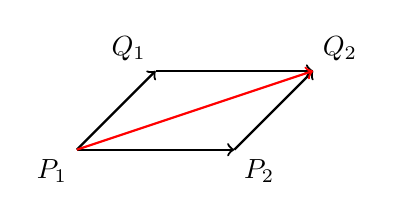
\begin{tikzpicture}
                \coordinate (P_1) at (0, 0);
                \coordinate (P_2) at (2, 0);
                \coordinate (Q_1) at (1, 1);
                \coordinate (Q_2) at (3, 1);
                \draw[thick, ->] (P_1) -- (P_2);
                \draw[thick, ->] (P_1) -- (Q_1);
                \draw[thick, ->] (Q_1) -- (Q_2);
                \draw[thick, ->] (P_2) -- (Q_2);
                \draw[red, thick, ->] (P_1) -- (Q_2);
                \node[below left] at (P_1) {\(P_1\)};
                \node[below right] at (P_2) {\(P_2\)};
                \node[above right] at (Q_2) {\(Q_2\)};
                \node[above left] at (Q_1) {\(Q_1\)};
            \end{tikzpicture}
        \end{center} 
\end{enumerate}
}

\dfn{Sottospazio affine}{Sia \(A_n(K)\) uno spazio affine. Si dice \textbf{sottospazio affine} di dimensione \(m \le n\) una struttura data da
\begin{enumerate}
    \item \(\emptyset \neq A' \subseteq A\), detto \textbf{sostegno del sottospazio affine} 
    \item \(V_m(K)\) sottospazio di \(V_n(K)\) 
    \item la restrizione dell'applicazione \(f\) ad \(A' \times A'\) troncata a \(V_m(K)\), purché questa sia ancora un'applicazione che gode delle proprietà elencate nella definizione di spazio affine
\end{enumerate}}

\dfn{Traslazione}{Fissato un vettore \(v \in V_n(K)\) si dice \textbf{traslazione}, individuata da \(v\), la corrispondenza \[
t_v: A \to A \quad e \quad P \to Q
\] che associa a un punto \(P \in A\) il punto \(Q\) traslato di \(P\) mediante il vettore \(v\).}

\paragraph{Osservazione:} \(\forall v \in V_n(K)\) la mappa \(t_v\) è una biiezione di \(A\), insieme di punti di \((A, V_n(K), f)\). E l'inversa di \(t_v\) è \(t_{-v}\).

\dfn{Sottospazio lineare}{Sia \(A_n(K)\) uno spazio affine. Si dice \textbf{sottospazio lineare} l'insieme dei traslati di un punto \(P\), detto \textbf{origine}, mediante i vettori \(v \in V_h(K) \le V_n(K)\), con \(h\) detta dimensione del sottospazio lineare. Inoltre si denota con \(S_h = [P, V_h(K)]\) il sottospazio lineare dato dal punto \(P\) e dallo spazio di traslazione \(V_h\).}

\dfn{Punti, rette, piani e iperpiani}{Sia \(A_n(K)\) uno spazio affine. Si dicono
\begin{itemize}
    \item \textbf{punti} i sottospazi lineari di dimensione 0 \[
            S_0 = [P, \{\ul{0} \} ] = \{P\} 
    \]
    \item \textbf{rette} i sottospazi lineari di dimensione 1 \[
            S_1 = [P, \mcL(v) ] \quad \text{con} \ v \neq \ul{0} \quad e \quad v \in V_n(K)
    \] 
    \item \textbf{piani} i sottospazi lineari di dimensione 2 \[
            S_2 = [P, \mcL(v_1, v_2) ] \quad \text{con} \ v_1, v_2 \neq \ul{0} \quad e \quad v_1, v_2 \in V_n(K)
    \] 
    \item \textbf{iperpiani} sono i sottospazi di dimensione \(n-1\)
\end{itemize}}
\mprop{}{Sia \(S_h = [P,V_h(K)]\) un sottospazio lineare di dimensione \(h\) sottospazio di \(A_n(K)\).
\begin{enumerate}
    \item siano \(Q, R \in S_h \implies \vec{QR} \in V_h(K)\) 
    \item se \(Q \in S_h\) e \(v \in V_h\), allora \(R = t_v (Q) \in S_h\)
\end{enumerate}}

\pf{Dimostrazione}{Dimostriamo entrambi i punti separatamente
\begin{enumerate}
    \item Per ipotesi \(Q \in S_h\), quindi \(Q = t_v(P)\) con \(v \in V_h(K)\). \(v = \vec{PQ} \in V_h\) e analogamente \(\vec{PR} \in V_h\). Ma allora \(\vec{QR} = \vec{QP} + \vec{PR} = - \vec{PQ} + \vec{PR} \in V_h\).
\begin{center}
        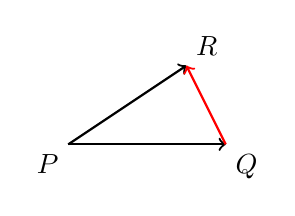
\begin{tikzpicture}
            \coordinate (P) at (0, 0);
            \coordinate (Q) at (2, 0);
            \coordinate (R) at (1.5, 1);
            \draw[thick, ->] (P) -- (R);
            \draw[thick, ->] (P) -- (Q);
            \draw[red, thick, ->] (Q) -- (R);
            \node[above right] at (R) {\(R\)};
            \node[below right] at (Q) {\(Q\)};
            \node[below left] at (P) {\(P\)};
        \end{tikzpicture}
\end{center}
    \item Poiché \(Q \in S_h, \ \vec{PQ} \in V_h\). Allora \(\vec{PR} + \vec{QR} = \vec{PQ} + \vec{v} \in V_h \implies \vec{PR} \in V_h\). Posto \(w = \vec{PR}\), \(t_w(P) = R\) con \(w \in V_h \implies R \in S_h\).
\begin{center}
        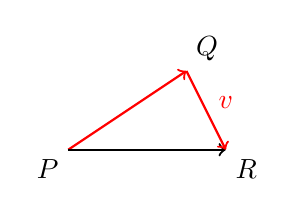
\begin{tikzpicture}
            \coordinate (P) at (0, 0);
            \coordinate (Q) at (2, 0);
            \coordinate (R) at (1.5, 1);
            \draw[red, thick, ->] (P) -- (R);
            \draw[thick, ->] (P) -- (Q);
            \draw[red, thick, ->] (R) -- (Q);
            \node[above right] at (R) {\(Q\)};
            \node[below right] at (Q) {\(R\)};
            \node[below left] at (P) {\(P\)};
            \node[red] at (2, 0.6) {\(v\)};
        \end{tikzpicture}
\end{center}
\end{enumerate}}

\mprop{}{Sia \(S_h=[P, V_h(K)]\) un sottospazio lineare di \(A_n(K)\). Ogni punto di \(S_h\) può essere scelto come origine di \(S_h\). Cioè dato \(Q \in S_h\) abbiamo che \([Q, V_h(K)] = S_h\).}

\pf{Dimostrazione}{Sia \(R \in S_h\). Allora \(\vec{PR} \in V_n\) e \(\vec{PQ}\in V_n\). Quindi \(\vec{QR} = \vec{QP} + \vec{PR} = - \vec{PQ} + \vec{PR} \in V_h \implies \vec{QR} \in V_h\).
\begin{center}
        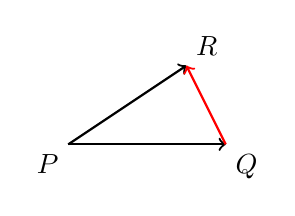
\begin{tikzpicture}
            \coordinate (P) at (0, 0);
            \coordinate (Q) at (2, 0);
            \coordinate (R) at (1.5, 1);
            \draw[thick, ->] (P) -- (R);
            \draw[thick, ->] (P) -- (Q);
            \draw[red, thick, ->] (Q) -- (R);
            \node[above right] at (R) {\(R\)};
            \node[below right] at (Q) {\(Q\)};
            \node[below left] at (P) {\(P\)};
        \end{tikzpicture}
\end{center}
Detto \(w = \vec{QR}\) abbiamo che \(R = t_v(Q)\). \(R\) è traslato di \(Q\) tramite il vettore \(w \in V_h \implies R \in [Q, V_h]\), quindi \[
    S_h \subseteq [Q, V_h]
\] con lo stesso ragionamento scambiamo \(P\) e \(Q\) si dimostra che  \[
[Q, V_h] \subseteq [P, V_h] = S_h
\] e ciò vale solo se \(S_h = [Q, V_h]\).}

\mprop{}{Siano \(S_h\) e \(S_k\) due sottospazi lineari di \(A_n(K)\). Allora \(S_h \subseteq S_k \iff S_h \cap S_k \neq \emptyset\) e \(V_h \le V_k\).}
\pf{Dimostrazione}{"\(\implies \)" Ovviamente \(S_h \cap S_k \neq \emptyset\) e sia \(P \in S_h \cap S_k\). Potremo scrivere \(S_h = [P, V_h]\) e \(S_k = [P, V_k]\). Sia \(v \in V_h\) e sia \(Q = t_v(P) \in S_h \subseteq S_k \implies Q \in S_k\) e sia \(Q = t_v(P)\) ovvero \(\vec{PQ}=v \in V_k \implies V_h \le V_k\).

"\(\impliedby \)" Sia \(P \in S_h \implies [P, V_h] \subseteq [P, V_k]\) (poiché per ipotesi \(V_h \subseteq V_k\)) \([P, V_h] = S_h\) e \([P, V_k]= S_k \implies S_h \subseteq S_k\).}

\mprop{}{Siano \(S_h\) e \(S_k\) sottospazi lineari di \(A_n(K)\). Sia \(S_h \cap S_k \neq \emptyset\) e sia \(P \in S_h \cap S_k\). Allora \[
        S_h \cap S_k = [P, V_h \cap V_k]
\] }

\pf{Dimostrazione}{Sia \(Q \in S_h \cap S_k\). Osserviamo che \(S_h = [P, V_h]\) e \(S_k = [P, V_k]\). \(Q = t_v(P)\) con \(v \in V_h\) (perché \(Q \in S_h\)). Ma \(Q = t_v(P)\) con \(v \in V_k\) (perché \(Q \in S_k\)). Quindi \(Q \in [P, V_h \cap V_k]\) perché \(v \in V_h \cap V_k\), cioè \[
        S_h \cap S_k \subseteq [P, V_h \cap V_k]
\] Viceversa dato \(Q = t_v(P)\) con \(v \in V_h \cap V_k \implies Q \) appartiene sia a \(S_h\) che ad \(S_k\), quindi \(Q \in S_h \cap S_k\), ovvero  \[
[P, V_h \cap V_k] \subseteq S_h \cap S_k
\] \[
\implies [P, V_h \cap V_k] = S_h \cap S_k
\] }

\dfn{Parallelismo tra sottospazi}{Due sottospazi lineari, \(S_p = [P, V_p]\) ed \(S_q = [Q, V_q]\), di \(A_n(K)\) si dicono \textbf{paralleli}, e si scrive \(S_p || S_q\), se i rispettivi spazi di traslazione sono confrontabili, ovvero quando \(V_p \subseteq V_q\), oppure \(V_q \subseteq V_p\).}

\paragraph{Osservazione 1:} La relazione di parallelismo non è transitiva. E' invece riflessiva e simmetrica. Non è quindi una relazione d'equivalenza.
\paragraph{Osservazione 2:} Due sottospazi lineari della stessa dimensione sono paralleli se, e soltanto se, hanno lo stesso spazio di traslazione. Quindi la relazione di parallelismo considerata tra spazi della stessa dimensione è una relazione d'equivalenza.

\mprop{}{Due sottospazi lineari paralleli e di uguale dimensione o coincidono oppure hanno intersezione vuota.}
\dfn{}{
\begin{itemize}
    \item Sia \(S=[P, V_1]\) una retta. Lo spazio \(V_1\) si dice \textbf{direzione} della retta \(S\). Quindi due rette sono parallele se, e soltanto se, hanno la stessa direzione
    \item Sia \(\pi = [P, V_2]\subseteq A_n(K)\) con \(n \ge 2\). Lo spazio \(V_2\) è detto \textbf{giacitura} di \(\pi\). Quindi due piani sono paralleli se, e soltanto se, hanno la stessa giacitura.
    \item Tre o più punti si dicono \textbf{allineati} se esiste una retta che li contiene tutti.
    \item Due o più rette si dicono \textbf{complanari} se esiste un piano che le contiene tutte.
\end{itemize}
}

\section{Proprietà di punti, rette e piani}
\mprop{}{In \(A_n(k)\), con \(n \ge 2\) 
\begin{enumerate}
    \item per ogni due punti distinti passa un'unica retta
    \item per due rette distinte, parallele o incidenti, passa un unico piano
    \item due rette complanari, aventi intersezione vuota, sono parallele
    \item per un punto passa un'unica retta parallela a una retta data (V Postulato di Euclide)
    \item per un punto passa un unico piano, parallelo ad un piano dato
    \item per tre punti, non allineati, passa un unico piano
    \item una retta, avente due punti distinti in un piano, giace nel piano
    \item per un punto passano almeno due rette distinte
\end{enumerate}}

\mprop{}{In \(A_3(K)\),
\begin{enumerate}
    \item una retta e un piano, aventi intersezione vuota, sono paralleli
    \item due piani, aventi intersezione vuota, sono paralleli
    \item due piani distinti, aventi in comune un punto, hanno in comune una retta per quel punto
    \item per una retta passano almeno due piani distinti
\end{enumerate}}

\dfn{Rette sghembe}{In \(A_n(K)\), con \(n \ge 3\), due rette non complanari si dicono \textbf{sghembe}.}
\mprop{}{In \(A_n(K)\), con \(n \ge 3\), esistono due rette \(r_1\) e \(r_2\) sghembe tra loro. Inoltre due rette sghembe \(r_1\) e \(r_2\), sono contenute su due piani \(\pi_1\) e \(\pi_2\) paralleli tra loro e distinti.}

\pf{Dimostrazione}{ Per ipotesi, \(A_n(K)\) ha dimensione almeno 3, quindi esistono nello spazio vettoriale  \(V_n(K)\) almeno 3 vettori linearmente indipendenti. Siano  essi \(u, v, w\). Siano inoltre, \(P\) un punto di \(A\) e \(Q\) il traslato di \(P\) mediante il vettore \(u\) (\(Q = t_u(P)\)). Dimostriamo che le rette \(r = [P, \mcL(v) ]\) ed \(s = [Q, \mcL(w) ]\) sono sghembe. Se infatti, esistesse un piano \(\pi = [P, V_2]\) che le contiene entrambe, lo spazio di traslazione di \(\pi \) conterrebbe 3 vettori linearmente indipendenti, cioè \(v, w\) e \(u = \vec{PQ}\) e ciò è un \textbf{assurdo!}
\begin{figure}[ht]
    \centering
    \def\svgwidth{0.3\columnwidth}
    \incfig{due-rette-complanari-con-3-vettori-linearmente-indipendenti}
    \label{fig:due-rette-complanari-con-3-vettori-linearmente-indipendenti}
\end{figure}
Siano ora \(t = [T, \mcL(v) ]\) e \(t' = [T', \mcL(v') ]\) due rette sghembe. I vettori \(v\) e \(v'\) generano uno spazio vettoriale \(V_2\) di dimensione 2. Pertanto, i piani  \(\pi = [T, V_2]\) e \(\pi' = [T', V_2]\), che risultano paralleli, sono distinti e contengono, rispettivamente le rette \(t\) e \(t'\).}

\section{Geometria analitica in \(A_n(\RR )\)}
\dfn{Riferimento affine}{Si dice \textbf{riferimento affine} di \(A_n(\RR )\) una coppia \(RA = [O,B]\) costituita da un punto \(O\) fissato, detto origine, e da una base \(B\) dello spazio vettoriale \(V_n(\RR )\).}

\dfn{Coordinate}{Fissato, in \(A_n(\RR )\), un riferimento affine \(RA = [O,B]\), si dicono \textbf{coordinate} del punto \(P\) in \(RA\) le componenti, in \(B\), del vettore \(\vec{OP}\) e si scrive \(P=(x_i)_{i \in I_n}\).}

\begin{enumerate}
\item In \(A_1(\RR )\), un riferimento affine è una coppia \(RA = [O,B]\), ove \(O\) è un punto fissato e \(B = (e_1)\) è una base di \(V_1(\RR )\). Se \(\vec{OP}=xe_1\), si scrive \(P=(x)\) e si dice che \(x\) è l'\textbf{ascissa} del punto \(P\) in \(RA\). 
\begin{figure}[ht]
    \centering
    \def\svgwidth{0.5\columnwidth}
    \incfig{ascissa}
    \label{fig:ascissa}
\end{figure}
\item In \(A_2(\RR )\), un riferimento affine è una coppia \(RA = [O,B]\), ove \(O\) è un punto fissato e \(B = (e_1, e_2)\) è una base di \(V_2(\RR )\). La retta \([O, \mcL(e_1) ]\) è detta \textbf{asse delle ascisse} e la retta \([O, \mcL(e_2) ]\) è detta \textbf{asse delle ordinate}. Se \(\vec{OP} = xe_1 + y e_2\), si scrive \(P = (x, y)\) e si dice che \((x,y)\) è la coppia delle coordinate di \(P\) in \(RA\), dette rispettivamente \textbf{ascissa} e \textbf{ordinata} del punto \(P\).
\begin{figure}[ht]
    \centering
    \incfig{ascissa-e-ordinata}
    \label{fig:ascissa-e-ordinata}
\end{figure}
\item In \(A_3(\RR )\), un riferimento affine è una coppia \(RA = [O,B]\), ove \(O\) è un punto fissato e \(B = (e_1, e_2, e_3)\) è una base di \(V_3(\RR )\). La retta \([O, \mcL(e_1) ]\) è detta \textbf{asse delle ascisse}, la retta \([O, \mcL(e_2) ]\) è detta \textbf{asse delle ordinate} e la retta \([O, \mcL(e_3) ]\) è detta \textbf{asse delle quote}. Sono detti \textbf{piani coordinati} i piani \(xy = [O, \mcL(e_1, e_2) ], xz = [O, \mcL(e_1, e_3) ]\) e \(yz = [O, \mcL(e_2, e_3) ]\). Inoltre, se \(\vec{OP}=xe_1+ ye_2 + ze_3\), si scrive \(P = (x, y,z)\) e si dice che \((x, y, z)\) è la terna delle coordinate di \(P\) in \(RA\), dette rispettivamente \textbf{ascissa, ordinata} e \textbf{quota} del punto \(P\).
\begin{figure}[ht]
    \centering
    \incfig{terne-di-coordinate}
    \label{fig:terne-di-coordinate}
\end{figure}
\end{enumerate}

\newpage
\thm{}{In \(A_n(K)\), con \(RA = [O, B]\), siano \(P = (x_1', x_2', \ldots , x_n')\) e \(Q = (x_1 '', x_2 '', \ldots  , x_n '')\) due punti di \(A\). Allora le componenti di \(\vec{PQ}\) rispetto a \(B\) sono \[
(x_1 '' - x_1', x_2 '' - x_2' , \ldots, x_n '' - x_n')
\] }

\pf{Dimostrazione}{Posti due vettori \[
\vec{OP} : \ x_1' e_1+ x_2' e_2 + \ldots + x_n' e_n
\] \[
\vec{OQ}: \ x_1 '' e_1 + x_2 '' e_2 + \ldots + x_n '' e_n
\]Per la proprietà della definizione di spazio affine possiamo dire che \[
\vec{PQ} = \vec{PO} + \vec{OQ} = \vec{OQ} - \vec{OP} = \sum_{i \in I_n} (x_i '' - x_i') e_i
\] }
Posti \[
 X '' = \begin{pmatrix} x ''_1 \\ x ''_2\\ \vdots \\ x ''_n \end{pmatrix}, X' = \begin{pmatrix} x'_1 \\ x'_2\\ \vdots \\ x'_n \end{pmatrix} \text{ e } T = \begin{pmatrix} t_1 \\ t_2\\ \vdots \\ t_n \end{pmatrix}
\] si ottiene l'equivalente, ma spesso più agevole, forma matriciale: \[
X '' - X' = T
\] che può essere riscritta come \[
X '' = X' + T
\] Da quest'ultima equazione si vede che le coordinate del traslato del punto \(P = (x_1', x_2', \ldots , x_n')\), attraverso il vettore \(v\) di componenti \((t_1, t_2, \ldots , t_n)\), si ottengono sommando, ordinatamente, alle coordinate di \(P\) le componenti del vettore di traslazione. Per questo le relazioni che compaiono nell'equazione sono anche dette \textbf{equazioni della traslazione individuata da \(v\)}.

\dfn{Punto medio}{Dato \(P\) e \(Q \in A\) (insieme dei punti di \(A_n(\RR )\)), definiamo il punto medio del segmento \([PQ]\) come \[
M = t_{1/2 \vec{PQ}} (P)
\] 
\begin{center}
    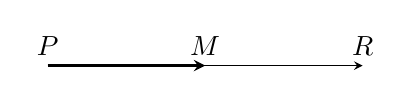
\begin{tikzpicture}
        \coordinate (P) at (0, 0);
        \coordinate (M) at (2, 0);
        \coordinate (R) at (4, 0);
        \draw[thick, -stealth] (P) -- (M);
        \draw[thin, -stealth] (P) -- (R);
        \node[above] at (R) {\(R\)};
        \node[above] at (M) {\(M\)};
        \node[above] at (P) {\(P\)};
    \end{tikzpicture}
\end{center}}

\mprop{}{Dati \(P, Q \in A\) e dato un riferimento affine \(RA = [O, B]\) abbiamo che le coordinate del punto medio di \(P\) e \(Q\) sono le semisomme delle coordinate omonime di \(P\) e di \(Q\).}

\dfn{Punto simmetrico}{In \(A_n(\RR )\) dati i punti \(P\) e \(C\) diremo che \(S\) è il \textbf{punto simmetrico} di \(P\) rispetto a \(C\) se \(C\) è il punto medio di \([P, S]\).}

\section{Rappresentazioni analitiche}
\dfn{Equazioni parametriche di una retta in \(A_n(\RR )\)}{Sia \(RA = [O,B]\) un riferimento fissato in \(A_n(\RR )\), ove \(B = (e_1, e_2, \ldots , e_n)\). Sia \(r = [P, V_1 = \mcL(v) ]\) la retta di origine il punto \(P = (x_1', x_2', \ldots , x_n')\) e spazio di traslazione generato da \(v = (l_1, l_2, \ldots , l_n)\). Il generico vettore \(w\) di \(\mcL(v) \) è proporzionale al vettore \(v\), cioè \(w = tv\), con \(t \in \RR \), quindi, \(w = (tl_1, tl_2, \ldots , tl_n)\). Dato che la retta \(r\) è il luogo dei traslati di \(P\) attraverso i vettori di \(\mcL(v) \), applicando le equazioni del teorema precedente si ottengono le coordinate del generico punto di \(r\) \[
\begin{cases}
    \ x_1 = x_1' + l_1t \\
    \ x_2 = x_2' + l_2t \\
    \ \ldots \ldots \ldots \ldots \\
    \ x_n = x_n' + l_nt \\
\end{cases} \quad \text{con} \quad t \in \RR , \quad (l_1, l_2, \ldots , l_n) \neq \ul{0} 
\] tali equazioni sono dette \textbf{equazioni parametriche} di \(r\) in \(A_n(\RR )\). Al variare di \(t \in \RR \), si ottengono le coordinate di tutti i punti di una retta e, quindi, tutti i punti di una retta sono \(\infty^{1}\).}

\dfn{Parametri direttori}{Si dicono \textbf{parametri direttori} di \(r = [P, V_1]\), le componenti di un qualunque vettore nullo di \(V_1\).}

\end{document}
